\chapter[Models and Theories]{Models and Theories of Dipoles Coupled to a Cavity}\label{ch:theory}

\section{Dipoles Coupled to a Cavity}
Light has been widely employed to transmit information since the first semiconductor laser was demonstrated by researchers from General Electric and MIT's Lincoln Laboratory in 1962~\cite{Keyes1962}, and an appropriate material for optical fibers was found by Kao and Hockham from International Telephone and Telegraph Company in 1966~\cite{Kao1966}. Light is also believed to be a good candidate for information processing to replace the present electronic processing~\cite{Nagy2006a,Hemmer2005}. A light beam does not interact with another light beam in general, however, which is a big barrier for light control and information processing.

Optical cavities capture light in a confined space and enhance the electromagnetical field through light-reflection and light-scattering, making the control of light easier (see Fig.~\ref{Cavity_withDipoleT}). In a semiconductor, which is the emitter of interest in this thesis, electrons and holes in the conduction band and valence band can controllably annihilate to emit a polarized photon. A bound electron and a hole pair produced by exciting an electron to the conduction band in a semiconductor material is called an exciton. Photon emission by exciton annihilation is generally a dipole quantum transition process. In an inverse process, light can also be absorbed through dipole excitation from a lower energy state to a higher excited state. Here, a dipole is an electronic oscillator which contains a charge oscillating in a electromagnetic field. The dipole approximation is used when the electromagnetic field is approximately constant within the range of electron displacement. In this study, the dipole approximation is always used.

\begin{figure}[htp]%[floatfix]
\centering
\begin{center}
%\DeclareGraphicsRule{.pdf}{eps}{}{`convert #1 eps:-}
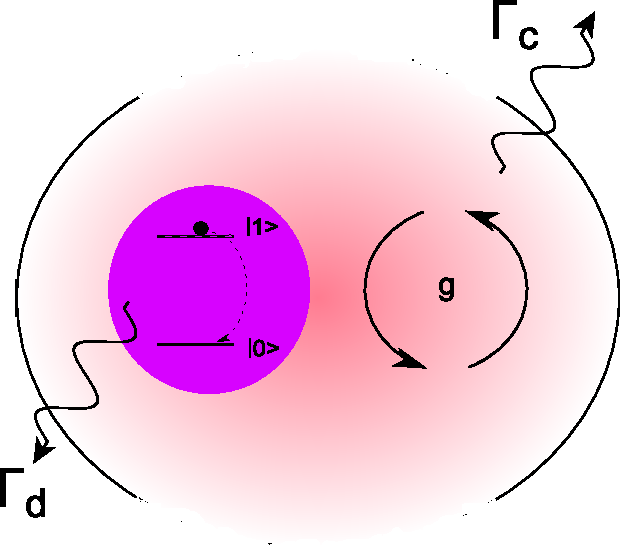
\includegraphics[width=7cm]{./Figs/Cavity_withDipoleT}%[bb=1.0in 1.0in 7.5in 10in]
\end{center}
\caption[A diagram of a cavity with one dipole.]{\textbf{A diagram of a cavity with one dipole.} }
\label{Cavity_withDipoleT}
\end{figure}


In addition to semiconductors, some light-emitting molecules, atoms and ions can also have dipole quantum transitions which emit photons. We also call the excited state of an emitter in those media an exciton, which is the basic unit of light emission~\cite{Gibbs2011}. A quantum dot (QD) is a good example of a photon emitter, in which the electrons are confined in a quantum box and discretely occupy energy levels where quantum transitions can occur under the drive of an external field. Particularly, we will consider the optical pump as a driver of light emission in this thesis.

A dipole can be viewed as a two-level system, which has a ground state of $\ket{0}$ and an excited state of $\ket{1}$. As the electron oscillates, it has a resonant frequency of $\Omega_d=(E_1-E_0)/\hbar$ and an optical moment or dipole moment of ${\bm\mu_d}$, where $E_1$ and $E_0$ are the eigen-energies of the excited and ground states respectively. The optical moment operator for the electron in the Heisenberg representation is defined as
\begin{equation}
\mathbf{\hat{d}}(t)=-e\mathbf{\hat{r}}(t),\label{eq:dt1}
\end{equation}
where $e$ is the unit charge, and $\mathbf{\hat{r}}$ is the position operator for the electron. The position operator determines the spatial distribution of charge and its time evolution. If we assume the dipole is in $\ket{\Psi}=1/\sqrt{2}(\ket{0}+\ket{1})$ at a given time $t=0$, the dipole moment can be measured as ${\bm\mu_d}=-e\bra{0}\mathbf{\hat{r}}\ket{1}$.  Considering a harmonic form of oscillation~\cite{Gerry2005,Mahan2000}, one can rewrite the optical moment operator as
\begin{equation}
\mathbf{\hat{d}}(t)={\bm\mu_d}[\hat{\sigma}_d^-(t=0) e^{-i(\Omega_d-i\Gamma_d/2) t} +\hat{\sigma}_d^+(t=0)e^{i(\Omega_d+i\Gamma_d/2) t}],\label{eq:dt2}
\end{equation}
where $\hat{\sigma}^{+/-}_d$ are Pauli operators for the exciton, and $\Gamma_d$ is the decay rate of dipole oscillation, which can be measured as the full-width-half-maximum (FWHM) of its spectrum. The $\hat{\sigma}^{+}_d$ operator is defined as $\hat{\sigma}^{+}_d=\ket{1}\bra{0}$, which moves a dipole from the ground state $\ket{0}$ to the excited state $\ket{1}$; in contrast, the $\hat{\sigma}^{-}_d$ operator is defined as $\hat{\sigma}^{-}_d=\ket{0}\bra{1}$, which moves a dipole from the excited state $\ket{1}$ to the ground state $\ket{0}$. Writing $\mathbf{\hat{d}}(\omega)=\int_{0}^{+\infty}{dt e^{i\omega t}\mathbf{\hat{d}}(t)}$, one obtains the quantum dipole moment operator in the frequency domain as
\begin{equation}
 \label{dipole}
  \mathbf{\hat{d}}(\omega) =
{i\bm\mu_d}\left [ \frac{\hat{\sigma}_d^-(t=0)}
{\omega-\Omega_d+i\Gamma_d/2}+\frac{\hat{\sigma}_d^+(t=0)}{\omega+\Omega_d+i\Gamma_d/2}\right ].
\end{equation}
%By comparing Equs.\eqref{eq:dt1} and~\eqref{eq:dt2}, one can obtain
%\begin{equation}
%{\bm\mu_d}=-e\bra{0}\mathbf{\hat{r}}\ket{1}.
%\end{equation}

In our study, the dipoles sit in the optical field of a cavity made by a semiconductor or many other media. Since the electrical field dominates the photon-dipole interactions in our case, we are only concerned with the electric field, or E-field. A cavity is usually characterized by its spectrum or power spectrum, which is defined as the Fourier transform of the modulus square of the time-domain field strength. One can identify the resonance of $\omega_c$ and the decay rate of $\Gamma_c$ in a certain mode. A mode is a defined pattern of the electromagnetic field for a cavity. The mode of a cavity is usually believed to be pre-determined by the bare cavity with a given geometric shape, but in this thesis we will show that the parameters (resonance and decay rate, or spectral width) of the cavity can be changed in the presence of photon emitters.

The mode of a bare cavity, where no photon emitters are added, can be calculated using some software, such as Lumerical Solutions~\cite{LumericalSolutions} based on FDTD method, which we used throughout the course of the research in this thesis.

%The interaction between dipoles and cavities can be


As nanophotonic innovation and nanotechnology march on, high-Q (optical quality) cavities can be achieved commonly~\cite{Akahane2003, Akahane2005}, and photon emitters can be implanted in a cavity accurately~\cite{Reithmaier2004, Reitzenstein2008}. As a result, some exciting or unexpected phenomena have been witnessed because of the interaction between a large number of individual emitters and a coupled optical cavity. For example, researchers have observed spectral broadening effects in InAs/InGaAs quantum dots (QDs) in a semiconductor photonic nanocavity~\cite{Tawara2008}. Meanwhile, cavity enhancement and spectral narrowing effect in nitrogen vacancy (NV) center(s), QD(s) and golden nano-particles have also been observed experimentally~\cite{Wolters2010, Faraon2011, Reithmaier2004, Englund2005, lodahl2004controlling}. An in-depth study of cavity-ensemble emission is used to explain these experimental phenomena and to predict new properties.

%\begin{figure}[H]
%\centering
%\begin{center}
%\includegraphics[width=8cm]{./Figs/pc}
%\end{center}
%\caption[Diagram of a Photonic Crystal H3 cavity with QDs.]{\textbf{Diagram of a Photonic Crystal H3 cavity with QDs.}  }
%\label{pc}
%\end{figure}

%\begin{figure}[H]
%\centering
%\begin{center}
%\includegraphics[width=8cm]{./Figs/Pillar_arrows}
%\end{center}
%\caption[Diagram of a micropillar cavity with QDs.]{\textbf{Diagram of a micropillar cavity with QDs.}  }
%\label{pillar}
%\end{figure}

%So far, however, theoretical studies on this topic are largely focused on few emitters coupled cavity luminescence~\cite{Hughes2009, Hughes2007, Xu2000, Averkiev2009}, or studied under truncated parameters by reducing an ensemble of emitters as one single emitter~\cite{Laussy2006, Reboul2009, Schwab2006, Illes2010a}, or studied without sophisticated considering the interaction between emitters~\cite{Meldrum2010}, and so on.

There are many models to explain the collective luminescence in a cavity field, but there are few based on the microscopic scattering process among a large number of emitters and the cavities. Rate equations and master equation (ME) methods are two widely used statistical methods suitable for a huge number of emitters and a few emitters cases~\cite{Hughes2009, Hughes2007, Xu2000, Averkiev2009}, respectively. Some phenomenological parameters, such as pumping rate, come from parameter fitting rather than first principles coefficients. Some of the ME methods only focused on one or two strongly coupled excitons~\cite{Laussy2006, Reboul2009, Schwab2006, Illes2010a}, and truncated the ensemble effect into phenomenological parameters. Other researchers try to adjust ME models to $N$-exciton coupled cavities~\cite{Illes2010a,Laussy2011}, but discussions are limited to a few excitons strongly coupled cavities, and these models can hardly explain the inhomogeneous broadening effect with a large number of background excitons, as we will discuss later. The ME-based Monte Carlo method and quantum trajectory method~\cite{Nowak2008,Meldrum2009,Temnov2005} have the same drawbacks of employing phenomenological parameters, and so far none has explicitly shown the spectral shifting effects.  A model based on Fermi's golden rule was developed by Meldrum to assess the spectral inhomogeneous broadening effect~\cite{Meldrum2010}, but it doesn't consider emitter-emitter interactions and hence may not be able to reflect well the spectral shifting effect. Among these models, moreover, it is still difficult to explain how light travels in the cavity and among the ensemble of photon emitters and hence revises the optical property of the cavity, as the models mainly focus on the energy transmission between levels and individuals, and assume that both the corresponding luminescence frequencies and modes are essentially determined by the bare cavity in which the photon emitters are not added.

As discussed in the introduction, the Green function method may be a good method to calculate ensemble effects in optical cavities. This chapter will introduce some basic features of the GF method and the models we are going to use in the remaining chapters. In the next section, we will first introduce the approach to calculate bare cavity GFs, and then discuss how to effectively calculate the GFs with $N$ dipoles. The initial conditions and the cavity spectrum calculation theory will be discussed next. The ME method will also be introduced at the end of this chapter.

%The initial motivation for the study throughout this thesis is to provide a general theory fully considering the interaction between emitters and cavity in linear region, and explain the detuning effect to cavity optical properties caused by coupled individual emitters, and how a cavity affects the interaction among emitters.

\section{Green Function Method of Optical Emission and Scattering}
This section will be introduced following the diagram in Fig.~\ref{FromG2S}.

\begin{figure}[htp]%[floatfix]
\centering
\begin{center}
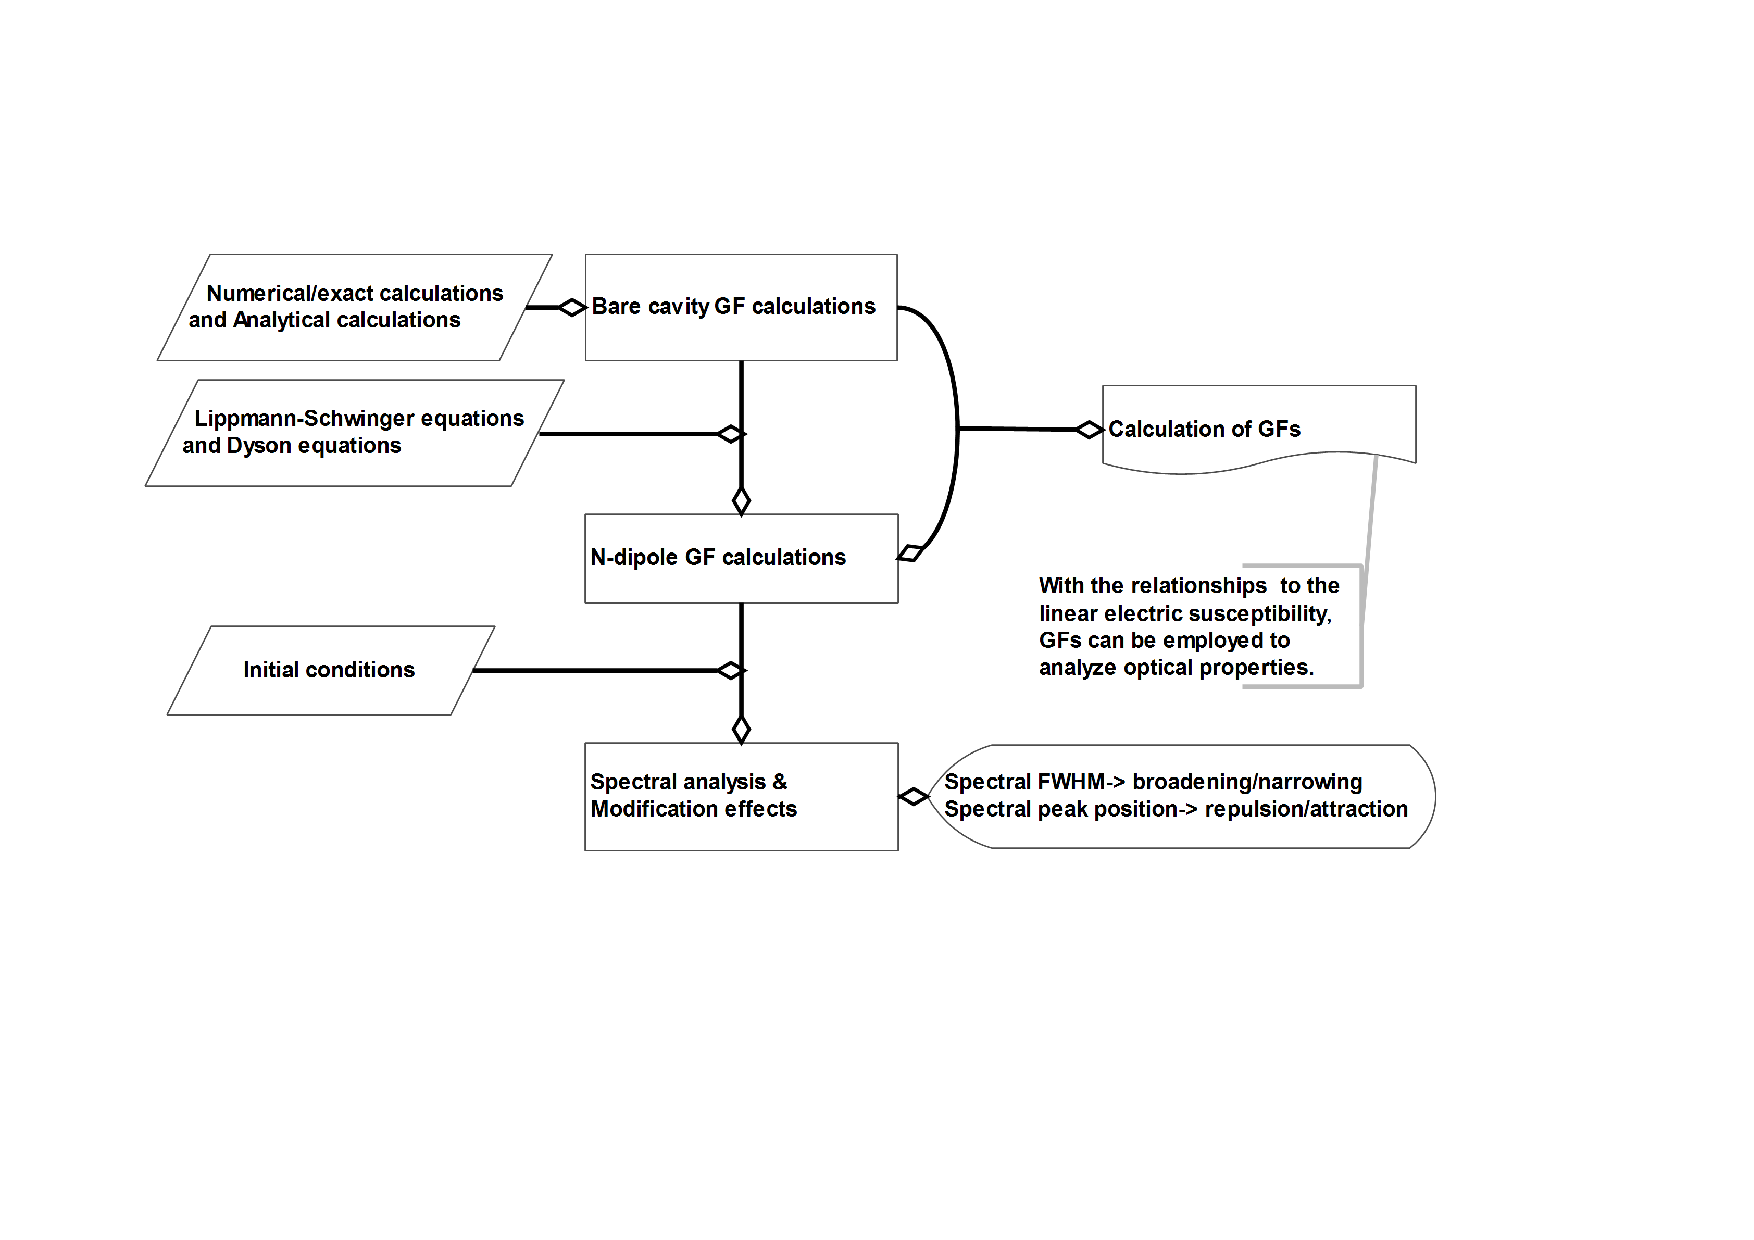
\includegraphics[width=16cm]{./Figs/FromG2S}%[bb=1.0in 1.0in 7.5in 10in]
\end{center}
\caption[The diagram of Green function theory for the exciton-cavity study.]{\textbf{The diagram of GF theory for the exciton-cavity study.} }
\label{FromG2S}
\end{figure}

\subsection{Classical GFT and FDTD method}\label{section:GFT}
In an optical cavity or a waveguide, corresponding to a given mode $\mathbf{f}_\lambda(\mathbf{r})$, the Maxwell equations give~\cite{Wubs2004}
\begin{equation}
 \label{eq:Maxwell}
-\nabla \times \nabla \times \mathbf{f}_\lambda(\mathbf{r}) + \varepsilon(\mathbf{r})(\omega_\lambda/c)^2 \mathbf{f}_\lambda(\mathbf{r}) = 0,
\end{equation}
where we have made $\lambda=(\mathbf{k},s)$, $k=\omega/c$, and $s$ is the polarization degenerate index (determined by the symmetry of the cavity or waveguide). Here, the mode $\mathbf{f}_\lambda(\mathbf{r})$ is
a harmonic solutions of the Maxwell equations for the inhomogeneous dielectric in absence of dipoles. If we put a dipole into the dielectric at ${\bf r}'$, there is a classical Green function tensor (GFT), $\Grrw$, detected at ${\bf r}$. $\varepsilon(\mathbf{r})$ is the permittivity of the medium at ${\bf r}$.
Notice that we limit our discussion of the GFTs to the frequency domain and only the electric GFTs--
the Magnetic GFTs, $\mathbf{G}_M(\rr, \omega)$ can be discussed similarly. The GFT corresponding to mode $\mathbf{f}_\lambda(\mathbf{r})$ is defined by a wave equation similar to Eq. (\ref{eq:Maxwell})
but with a dipole source  (generally a polarized source, described by a delta or Lorentzian function, based on the dipole approximation)
on the right-hand side, which is given by
\begin{equation}
\label{def:GEwave}
 -\nabla \times \nabla \times \mathbf{G}(\rr,\omega) + \varepsilon(\mathbf{r})(\omega/c)^2 \mathbf{G}(\rr,\omega) = \mathbf{I} \delta \left(\br-\br'\right).
\end{equation}
The GFT defined above describes how the wave propagates from source $\mathbf{r}'$ to detector $\mathbf{r}$. The total GFT can be decomposed into transverse and longitudinal parts, $\mathbf{G}^T(\rr,\omega)$ and $\mathbf{G}^L(\rr,\omega)$, respectively. That is,
\begin{equation}
\mathbf{G}(\rr,\omega)=\mathbf{G}^T(\rr,\omega)+\mathbf{G}^L(\rr,\omega),
\end{equation}
where the longitudinal part is given by~\cite{Wubs2004}
\begin{equation}
\label{GL}
\mathbf{G}^L(\rr,\omega)=\frac{\boldsymbol{\delta}_{\varepsilon}^L \left(\br',\br\right)}{\varepsilon(\mathbf{r})(\omega_\lambda/c)^2}.
\end{equation}
The $\boldsymbol{\delta}_{\varepsilon}^L \left(\br',\br\right)$ in the equation above is the generalized longitudinal delta function in a dielectric medium, and is defined as the difference between the ordinary Dirac, $\mathbf{I} \delta \left(\br-\br'\right)$,
and the generalized transverse delta function, $\boldsymbol{\delta}_{\varepsilon}^T \left(\br',\br\right)$. The transverse delta function is defined as
\begin{equation}
\boldsymbol{\delta}_{\varepsilon}^T \left(\br,\br'\right)
=\sum_{\lambda}{\mathbf{f}_\lambda^*(\mathbf{r})\mathbf{f}_\lambda(\mathbf{r}') \varepsilon(\mathbf{r}')},
\end{equation}
and has the projection property $\int{d\br' \boldsymbol{\delta}_{\varepsilon}^T \left(\br',\br\right) \cdot \mathbf{X}^T(\br')}=\mathbf{X}^T(\br)$ for any transverse vector field  $\mathbf{X}^T(\br)$.
In Equ.\eqref{GL}, the generalized longitudinal delta function in a dielectric medium, $\delta_{\varepsilon}^L \left(\br-\br'\right)$, and hence $\mathbf{G}^L(\rr,\omega)$ gives a countable effect only when $\br=\br'$. In most cases in this thesis referring to high-Q cavities, one can approximate the total GFT by the transverse GFT, which means
\begin{equation}
\mathbf{G}(\rr,\omega) \approx \mathbf{G}^T(\rr,\omega),
\end{equation}
which can be a Lorentzian function, as will be discussed in Section~\ref{section:Lorentz} and Appendix~\ref{App:analyticalGF}.

If the background E-field at $\br$ is $\mathbf{E}_0$, then the E-field at $\br$ responding to a polarized source at $\br'$ is given by
\begin{equation}
 \label{EandGwithE0}
\mathbf{E}=\mathbf{E}_0+\mathbf{G} \cdot \mathbf{P},
\end{equation}
where $\mathbf{P}$ is the source's polarization vector or polarization density.
Now, we let $\mathbf{E}_0=0$, which means there is no initial E-field at the detector's position.
Hence, one has
\begin{equation}\label{eq:EGP}
\mathbf{E}=\mathbf{G} \cdot \mathbf{P}.
\end{equation}
In terms of matrices, the equation above can be written as
\begin{align}
\label{EandGwithoutE0}
\left( \begin{array}{c}
       E_x\\
       E_y\\
       E_z  \end{array} \right)
                   = \left( \begin{array}{c}
                      G_{xx} \quad G_{xy} \quad G_{xz} \\
                      G_{yx} \quad G_{yy} \quad G_{yz} \\
                      G_{zx} \quad G_{zy} \quad G_{zz}  \end{array}  \right) \left( \begin{array}{c}
                                                                                     P_x\\
                                                                                     P_y\\
                                                                                     P_z
                                                                                    \end{array} \right).
\end{align}
If we let the polarization source only have $x$ component or orientate the polarized source to $x$ direction, which means
\begin{equation}
 \label{Px}
\mathbf{P}=\left( \begin{array}{c}
                   P_x\\
                   0\\
                   0
                  \end{array} \right),
\end{equation}
then only the first column of GFT contributes to the measured E-field, and from Eq. (\ref{EandGwithoutE0}) we obtain
\begin{equation}
 \label{Gix}
G_{ix} \equiv \frac{E_{i}}{P_x}, \quad (i=x, y, z).
\end{equation}
The $G_{ix}\,(i=x, y, z)$ stretch out the first column of the GFT.
Similarly, if we orientate the polarized source to $y$ and $z$ direction, we can get the second and third column of GFT.
All the discussions above form the basis of the FDTD method to obtain GFT for our configuration.


The FDTD method is a numerical method to calculate the time domain electromagnetic field propagating in an arbitrary optical structure.
Further, we can get frequency domain results by operating a Fourier transformation from the time domain fields,
and get the background Green function tensor components as
\begin{equation}
 \label{def:GFT}
 G_{ij}(\rr,\omega)=\frac{{\rm FT}[E^i_\lambda(\mathbf{r},t)]}{{\rm FT}[E^j_d(\mathbf{r}',t)]}
=\frac{E^i_\lambda(\mathbf{r},\omega)}{E^j_d(\mathbf{r}',\omega)}, \quad (i,j=x, y, z),
\end{equation}
where we assume the test dipole source is located at $\mathbf{r}'$ and only has a $j$ component of polarized electric field $E^j_d(\mathbf{r}')$
(we have replaced $ \mathbf{P}$ with $\mathbf{E}_d$, which is the observed E-field at the source and already includes the dielectric effect),
and the detector is located at $\mathbf{r}$ with $i=x, y, z$ components of electric field $E^i_\lambda(\mathbf{r})$, ${\rm FT}$ indicates Fourier transformation.
When we apply this formula in a waveguide or a cavity, the electric field $\mathbf{E}_\lambda$ here
can be the electric mode $\mathbf{f}_\lambda$ used above.

If $\br=\br'$, the real part of the Green function usually diverges~\cite{Dung2003}. We can use the imaginary part to identify the Green function:
\begin{equation}
 \label{GFTimag}
 {\rm Im}(G_{ij}(\br',\br',\omega))={\rm Im}\left(\frac{{\rm FT}[E^i_\lambda(\mathbf{r}',t)]}{{\rm FT}[E^j_d(\mathbf{r}',t)]}\right)
={\rm Im}\left(\frac{E^i_\lambda(\mathbf{r}',\omega)}{E^j_d(\mathbf{r}',\omega)}\right),
\end{equation}
where ${\it Im}$ means the imaginary part of a quantity.



For a dipole source $\mathbf{r}'=\mathbf{r}_d$ in an FDTD calculation (if using Lumerical Solutions~\cite{LumericalSolutions}), we have
\begin{equation}
 \label{def:dipleft}
E^j_d(\mathbf{r}_n,t)=-\frac{\mu_n^j}{\varepsilon_0}\exp(-2\ln(2)\frac{(t-t_0)^2}{\tau^2})\cdot\sin[\omega_0(t-t_0)],\quad j=x, y, z,
\end{equation}
where $\mu_n^j$ is the $j$th component of the dipole moment in a Cartesian coordinate, $t_0$ is the time delay of the dipole source,
and $\tau$ is the FWHM of the dipole pulse. Equ.~\eqref{def:dipleft} shows that the dipole oscillates at mode $\omega_0$ with a Gaussian amplitude profile in the time domain. So, through Fourier transformation, we can get
\begin{equation}
 \label{dipolefw}
E^j_d(\mathbf{r}_n,\omega)={\rm FT}[E^j_d(\mathbf{r}_n,t)].
\end{equation}

In practice, one can run an FDTD calculation in Lumerical, for example, and follow the steps listed in Appendix \ref{App:FDTD_GFT} to calculate the background or bare cavity GFTs.

Note that, in the linear optics of dielectric material, we have~\cite{Boyd2003}
\begin{equation}
\mathbf{P}=\varepsilon_0\mathbf{\chi} \cdot \mathbf{E},
\end{equation}
or
\begin{equation}\label{eq:polarization}
\mathbf{E}=\frac{1}{\varepsilon_0}\mathbf{\chi}^{-1} \cdot \mathbf{P},
\end{equation}
where $\mathbf{\chi}$ is the electric susceptibility of the medium.
By comparing Equ.\eqref{eq:EGP} with the linear polarization equation above, one can find that Equ.\eqref{eq:EGP} is identical to the linear optical polarization equation by defining
\begin{equation}
\mathbf{G}\equiv \frac{1}{\varepsilon_0}\mathbf{\chi}^{-1}.
\end{equation}
This relationship above shows that the GF method we use in this thesis corresponds to a linear optics model for a given optical structure. Moreover, once we obtain the GFs, we equivalently know the $\mathbf{\chi}$. Since $\mathbf{\chi}$ determines the optical properties such as dispersion, absorption, resonant shift and spectral broadening~\cite{Boyd2003,Cohen-Tannoudji1998,Haug1990,Maier2007,Novotny2006,Gerry2005,Sakoda2005}, we can analyze the optical properties of a given optical structure through calculating the GFs. In this study, we focus on the spectral behavior including resonant shift and spectral broadening effects of optical cavities with many dipoles.

%%%%
\subsection{Quantum Description of an Optical Cavity with $N$ Dipoles}
%In the scale of an atom, interactions should be described by full quantum operators in principle.
In a lossless cavity, to describe quantized light emission in an arbitrary inhomogeneous dielectric with relative dielectric function $\varepsilon(\mathbf{r})$ and a finite number N of embedded
dipoles in it, we employ a canonical Hamiltonian in the absence of dephasing and decoherence \cite{Vats2002,Wubs2004}:
\begin{equation}
\label{eq:h}
\begin{split}
 \hat{H} =& \hat{H}_{X}+\hat{H}_F+\hat{H}_I\\
=& \sum_n\hbar \Omega_n \hat{\sigma}_n^+\hat{\sigma}_n^-+
\sum_\lambda\hbar \omega_\lambda
\hat{a}_\lambda^\dagger\hat{a}_\lambda +\sum_{n,\lambda}(
\hat{\sigma}_n^- + \hat{\sigma}_n^+)(g_{n\lambda}
\hat{a}_\lambda+g_{n\lambda}^*\hat{a}_\lambda^\dagger),\\
\end{split}
\end{equation}
where the dipole is at the spatial position $\mathbf{r}_n$; $\hat{a}_{\lambda}^{\dagger}$ and $\hat{a}_{\lambda}$ represent the field mode operators to give the field Hamiltonian $\hat{H}_F=\sum_\lambda\hbar \omega_\lambda
\hat{a}_\lambda^\dagger\hat{a}_\lambda$; $\hat{\sigma}^{+/-}_n$ are the Pauli operators of the excitons
(for excitons that are in the frequency regime of interest) to give the exciton Hamiltonian $\hat{H}_{X}=\sum_n\hbar \Omega_n \hat{\sigma}_n^+\hat{\sigma}_n^-$;
the remaining exciton-photon interaction terms are treated within the dipole approximation
($\hat{H}_I=-\sum_n{\bm{\mu} _n \cdot \hat{\mathbf{E}}(\mathbf{r}_n)}$ corresponding to $\delta$-form polarization
\begin{equation}\label{eq:P}
\hat{\mathbf{P}}_n(\mathbf{r},t)=\delta(\mathbf{r}-\mathbf{r}_n)\bm{\mu} _n(\hat{\sigma}_n^- + \hat{\sigma}_n^+),
\end{equation}
valid for photon emitters whose spatial size is much smaller than a wavelength); we have assumed that there is no decay for individual dipole oscillation. The time dependence is implicit in the Heisenberg picture, and all derivations are under the approximation of single excitation.
In addition, $\Omega_n$ is the resonant frequency of the $n$th exciton, and $\omega_\lambda$ is the eigenfrequency
corresponding to the bare cavity modes of the system ($\mathbf{f}_\lambda(\mathbf{r})$) excluding the dipoles. The coupling strength between the dipole at $\br_n$ and the cavity mode field is given by~\cite{Wubs2004}
\begin{equation}
g_{n\lambda}=-i\sqrt{\frac{\hbar\omega_\lambda}{2 \varepsilon_0}}\boldsymbol{\mu}_n\cdot \mathbf{f}_\lambda(\mathbf{r}_n).
\end{equation}

The Heisenberg equations of motion for the operators can be derived from  $\dot {\hat O}_i = -i{\hbar^{-1}[\hat O_i,H]}$,
yielding~\cite{Wubs2004}
\begin{align}
\frac{d\hat{a}_\lambda}{dt}&=-i\omega_\lambda \hat{a}_\lambda-i\sum_n\hbar^{-1}g_{n\lambda}^*(\hat{\sigma}_n^-+\hat{\sigma}_n^+), \label{eq:a-t}\\
%
\frac{d\hat{a}_\lambda^\dagger}{dt}&=i\omega_\lambda \hat{a}_\lambda^\dagger+i\sum_n\hbar^{-1}g_{n\lambda}(\hat{\sigma}_n^-+\hat{\sigma}_n^+), \label{eq:a+t}\\
%
\frac{d\hat{\sigma}_n^-}{dt}&=-i\Omega_n\hat{\sigma}^-_n-i\hbar^{-1}\sum_{\lambda}(g_{n\lambda}
\hat{a}_\lambda+g_{n\lambda}^*\hat{a}_\lambda^\dagger), \label{eq:sig-t} \\
%
\frac{d\hat{\sigma}_n^+}{dt}&=i\Omega_n\hat{\sigma}^+_n+i\hbar^{-1}\sum_{\lambda}(g_{n\lambda}
\hat{a}_\lambda+g_{n\lambda}^*\hat{a}_\lambda^\dagger). \label{eq:sig+t}
%
%\frac{d\hat{\sigma}_{nz}}{dt}&=2i\hbar^{-1}\sum_{\lambda}(\hat{\sigma}_n^-- %\hat{\sigma}_n^+)(g_{n\lambda}
%\hat{a}_\lambda+g_{n\lambda}^*\hat{a}_\lambda^\dagger).
\end{align}

Next we perform a Laplace transform to positive frequency space,
$O(\omega)=\int_0^\infty dt e^{i\omega t}\, O(t)$, and obtain \cite{Wubs2004}:
\begin{align}
{\hat{a}_\lambda(\omega)}&= \hat{a}_\lambda(t=0) + \frac{i\hbar^{-1}}{\omega-\omega_\lambda}
\sum_n g_{n\lambda}^*[\frac{\hat{\sigma}_n^-(t=0)}{\omega-\omega_\lambda}
+\frac{\hat{\sigma}_n^+(t=0)}{\omega+\omega_\lambda}]\nonumber\\
& \quad + \frac{\hbar^{-2}}{\omega-\omega_\lambda}
\sum_{n,\lambda'} \frac{2g_{n\lambda}^*\Omega_n}{\omega^2-\Omega_n^2} [g_{n\lambda'}
\hat{a}_{\lambda'}(\omega)+g_{n\lambda'}^*\hat{a}_{\lambda'}^\dagger(\omega)], \label{eq:aw} \\
{\hat{a}_\lambda^\dagger(\omega)}&=\adag_\lambda(t=0) - \frac{i\hbar^{-1}}{\omega-\omega_\lambda}
\sum_n g_{n\lambda}^*[\frac{\hat{\sigma}_n^-(t=0)}{\omega-\omega_\lambda}
-\frac{\hat{\sigma}_n^+(t=0)}{\omega+\omega_\lambda}]\nonumber\\
& \quad + \frac{\hbar^{-2}}{\omega+\omega_\lambda}
\sum_{n,\lambda'} \frac{2g_{n\lambda}\Omega_n}{\omega^2-\Omega_n^2} [g_{n\lambda'}
\hat{a}_{\lambda'}(\omega)+g_{n\lambda'}^*\hat{a}_{\lambda'}^\dagger(\omega)],
\label{eq:adaggerw} \\
\hat{\sigma}_n^-(\omega)&=\frac{i\hat{\sigma}_n^-(t=0)}
{\omega-\Omega_n}+\frac{\hbar^{-1}}{\omega-\Omega_n}
\sum_{\lambda}[g_{n\lambda}
\hat{a}_\lambda(\omega)+g_{n\lambda}^*\hat{a}_\lambda^\dagger(\omega)], \label{eq:sig-w} \\
\hat{\sigma}_n^+(\omega)&=\frac{i\hat{\sigma}_n^+(t=0)}
{\omega+\Omega_n}-\frac{\hbar^{-1}}{\omega+\Omega_n} \sum_{\lambda}[g_{n\lambda}
\hat{a}_\lambda(\omega)+g_{n\lambda}^*\hat{a}_\lambda^\dagger(\omega)]. \label{eq:sig+w}
%\hat{\sigma}_{nz}(\omega)&=\frac{i\hat{\sigma}_{nz}(t=0)}
%{\omega}+\frac{2\hbar^{-1}\mu_n\hat{E}_\mu(\mathbf{r}_n)\ast
%[\hat{\sigma}_{n}^-(\omega)-\hat{\sigma}_{n}^+(\omega)]}{\omega}.
\end{align}
%
Here,
\begin{equation}
 \label{eq:Esum}
 \mathbf{\hat{E}}(\mathbf{r},t)=\mathbf{\hat{E}}^+(\mathbf{r},t)+\mathbf{\hat{E}}^-(\mathbf{r},t)=i\sum_\lambda\sqrt{\frac{\hbar
\omega_\lambda}{2\varepsilon_0}}\hat{a}_\lambda(t)\mathbf{f}_\lambda(\mathbf{r})+h.c.
\end{equation}
where the mode expansion of the inhomogeneous field operator $\mathbf{\hat{E}}$
has a sum of a positive-frequency part $\mathbf{\hat{E}}^+$ (containing only annihilation operators in the time domain or positive frequency components in the frequency domain through Fourier transformation)
and its Hermitian conjugate $\mathbf{\hat{E}}^-$, where
\begin{equation}
 \label{eq:E^plus}
 \mathbf{\hat{E}}^+(\mathbf{r},t)=i\sum_\lambda\sqrt{\frac{\hbar\omega_\lambda}{2\varepsilon_0}}\hat{a}_\lambda(t)\mathbf{f}_\lambda(\mathbf{r}).
\end{equation}
Notice that $\mathbf{\hat{E}}(\mathbf{r},t)$ here is equal to a non-interacting (no dipoles embedded) electric field operator everywhere, except at the positions $\mathbf{r}_n$ of the dipoles,
since the dipoles couple to fields in which their own polarization fields are included.
When we use $\mathbf{\hat{E}}(\mathbf{r}_n,t)$ at the dipole position $\mathbf{r}_n$,
it means a self-interaction polarization is included in the dipole self-coupling field; otherwise such a distinction is not necessary.


Using  Equ.\eqref{eq:aw} and~\eqref{eq:adaggerw}, and the expansion of $\mathbf{\hat{E}}$ (Equ.\eqref{eq:Esum}),
we obtain the electric field operator \cite{Wubs2004}:
%
\begin{subequations}
\label{eq:ew1_1}
\begin{align}
\mathbf{\hat{E}}(\mathbf{r},\omega) =& \mathbf{\hat{E}}^{(0)}(\mathbf{r},\omega)\label{bareE0_1}\\
&+ \sum_n{\mathbf{K}(\mathbf{r},\mathbf{r}_n,\omega)\cdot\hat{\mathbf{S}}_n(\omega)}\label{sourceE_1}\\
&+ \sum_n{\mathbf{K}(\mathbf{r},\mathbf{r}_n,\omega)\cdot\mathbf{U}_n(\omega)\cdot\mathbf{\hat{E}}(\mathbf{r}_n,\omega)}\label{scatteringE_1}
\end{align}
\end{subequations}
%
\begin{equation}
 =\mathbf{\hat{E}}^{(0)}(\mathbf{r},\omega)+ \mathbf{\hat{E}}_{source}(\mathbf{r},\omega)+\mathbf{\hat{E}}_{scatt}(\mathbf{r},\omega)\label{eq:E0sourcescatt_1},
% This is an important equation.
\end{equation}
where $\mathbf{K}(\mathbf{r},\mathbf{r}',\omega)$ is the Green function in the context of quantum description, $\hat{\mathbf{S}}_n(\omega)$ is the source operator, and $\mathbf{U}_n(\omega)$ is the scattering potential. The $\mathbf{K}(\mathbf{r},\mathbf{r}',\omega)$ can be defined as a dyadic quantity or a tensor by
\begin{equation}
 \label{K}
 \mathbf{K}(\mathbf{r},\mathbf{r}',\omega)=c^2\sum_\lambda\frac{\mathbf{f}_\lambda(\mathbf{r})\mathbf{f}_\lambda^*(\mathbf{r}')}
{(\omega^2-\omega_\lambda^2)}\frac{\omega_\lambda^2}{\omega^2},
\end{equation}
where we have assumed that the dipole moments are real and  we
have exploited the fact that the summation over $\lambda$ includes
contributions from $\mathbf{f}_\lambda$ and $\mathbf{f}_\lambda^*$ (per $\lambda$)
in the sum.
%(both are solutions
%of an equivalent eigenvalue problem).

Equ.\eqref{eq:ew1_1} is an exact Lippmann-Schwinger equation, and it describes the scattering of and emission by dipoles inside an inhomogeneous dielectric, both for strong and weak dipole-field interactions\footnote{The strong coupling occurs when the dipole-field coupling strength (which is half the Rabi frequency), is faster than any underlying dissipative rate and larger than $1/\tau$ where $\tau$ is the interaction time~\cite{Kimble1998}.}.
More clearly, we can represent the Lippmann-Schwinger equation as three parts (as shown in Equ.\eqref{eq:E0sourcescatt_1}): an undisturbed term
(first term), a source term (second term), and a scattering term (third term).


For the first term, Equ.\eqref{bareE0_1}, the operator $\mathbf{\hat{E}}^{(0)}(\mathbf{r},\omega)$ is the electric field in the absence of the dipoles, with both the positive and negative frequency parts and only depends on input light.


The term (\ref{sourceE_1}), corresponding to $\mathbf{\hat{E}}_{source}(\mathbf{r},\omega)$ in (\ref{eq:E0sourcescatt_1}) account for the field radiated by the dipoles. It is a sum of every dipole with a product of Green function tensor and an emitting source operator $\hat{\mathbf{S}}_n(\omega)$,
which is a vector and has the form $\mathbf{e}_n\hat{S}_n(\omega)$ in the direction of the atomic or exciton's dipole moment \cite{Wubs2004}, and
\begin{equation}
 \label{source}
 \hat{S}_n(\omega) \equiv \left(\frac{i\mu_n\omega^2}{\varepsilon_0c^2}\right)
\lbrack\frac{\hat{\sigma}_n^-(t=0)}{\omega-\Omega_n}+\frac{\hat{\sigma}_n^+(t=0)}{\omega+\Omega_n}\rbrack
=\frac{\omega^2}{\varepsilon_0c^2}\hat{d}_n(\omega),
\end{equation}
where we have plugged in Equ.\eqref{dipole} with $\Gamma_n=0$.
Since both Equ.\eqref{source} and Equ.\eqref{dipole} only depend on $\hat{\sigma}^{+/-}_n$, the Pauli operators of the excitons,
we can see that the second term includes the dipoles and its function is to describe emitting sources.
The initial expectation value of this term can be obtained if we know the initial states and the $n$th dipole's optical momentum \(\boldsymbol{\mu}_n\).

The term (\ref{scatteringE_1}), corresponding to $\mathbf{\hat{E}}_{scatt}(\mathbf{r},\omega)$ in (\ref{eq:E0sourcescatt_1}), contains two parts in every element of the summation for every dipole:
the optical potentials $\mathbf{U}_n(\omega)$ produced at the on-site dipole
and the initial electric operator $\mathbf{\hat{E}}(\mathbf{r}_n,\omega)$ measured at the corresponding dipole position $\mathbf{r}_n$.
$\mathbf{U}_n(\omega)$ is a dyadic and
\begin{equation}
 \label{Udyadic}
\mathbf{U}_n(\omega)=\mathbf{e}_nU_n(\omega)\mathbf{e}_n,
\end{equation}
 where
\begin{equation}
 \label{Un}
 U_n(\omega) \equiv \left(\frac{\mu_n^2\omega^2}{\hbar\varepsilon_0c^2}\right)
\left(\frac{2\Omega_n}{\Omega_n^2-\omega^2}\right),
\end{equation}
and
\begin{subequations}\label{directproduct}
\begin{align}
\mathbf{e}_n\mathbf{e}_n=& \mathbf{e}_n \otimes \mathbf{e}_n\\
=& \left( \! \begin{array}{cc}
    e_n^x \\ e_n^y \\ e_n^z
   \end{array} \! \right)
\left(\, e_n^x\quad e_n^y \quad e_n^z \, \right)=\left( \! \begin{array}{c}
                                  e_n^xe_n^x\quad  e_n^xe_n^y\quad  e_n^xe_n^z\\
                                  e_n^ye_n^x\quad  e_n^ye_n^y\quad  e_n^ye_n^z \\
                                  e_n^ze_n^x\quad  e_n^ze_n^y\quad e_n^ze_n^z
                                 \end{array} \! \right)
\end{align}
\end{subequations}
is the tensor direct product.
Correspondingly, if we omit the factor $(\frac{\omega^2}{c^2})$, we can have the polarization
\begin{equation}
 \label{alpha}
 \alpha_n(\omega) \equiv \frac{\mu_n^2}{\hbar\varepsilon_0}\,\frac{2\Omega_n}{\Omega_n^2-\omega^2},
\end{equation}
which is directly connected to the dipole polarization tensor or dyadic
${\bm \alpha}_n(\omega) = {\bf e}_n \alpha_n(\omega){\bf e}_n$. Whether you prefer to use $\mathbf{U}_n(\omega)$ or ${\bm \alpha}_n(\omega)$,
this part of the term strongly depends on the resonant frequencies $\pm\Omega_n$ and will become sharp and change sign when $\omega$ goes through the dipole resonances.
The electric field operator can set to be the initial background (cavity) electric field operator, with the form as shown in Equ. (\ref{eq:Esum}).
The initial expectation value of this operator can be calculated
according to the given initial dressed states (actually, the cavity's or photons' parts) and normalized modes $\mathbf{f}_\lambda$ at $\mathbf{r}_n$.
Considering all these effects, in terms of physics, we call it the scattering term.


Now, $\Krrw$ is a quantum Green function tensor defined from a fully quantized Lippmann-Schwinger equation~\cite{Wubs2004}.
According to Wubs's work~\cite{Wubs2004}, there are simple relationships among the quantum Green function tensor, $\Krrw$, the classical transverse Green function tensor, $\GTrrw$, and the classical total Green function, $\Grrw$, which we discussed in the last section:
\begin{equation}
 \label{KG}
 \Krrw=\Grrw+\frac{\mathbf{I}\delta(\mathbf{r}-\mathbf{r}')}{\varepsilon(\mathbf{r})(\omega/c)^2}
=\GTrrw+\frac{\bm{\delta}^T(\rr)}{\varepsilon(\mathbf{r})(\omega/c)^2},
\end{equation}
where $\mathbf{I}$ is the unit dyadic, and $\bm{\delta}^T(\rr)
=\sum_\lambda{\mathbf{f}_{\lambda}(\mathbf{r})\mathbf{f}_{\lambda}^*(\mathbf{r}')}\varepsilon(\mathbf{r})$
is a generalized transverse delta function. Notice that the factor $(\omega/c)^2$ is ignored in some publications (for example, see Ref.~\cite{Yao2009a,Hughes2007}).

According to this relationship,  the dyadic $\Krrw$ differs from the total Green function tensor of the medium and its transverse component only when its two position arguments $\mathbf{r}$ and $\mathbf{r}'$ coincide.
%Although different from $\mathbf{G}$, the quantity $\mathbf{K}$ will also be called a Green function.
Because of this, we can make $\mathbf{K}=\mathbf{G}$ in most situations without any problem,
and through calculating the classical Green function to equivalently obtain $\mathbf{K}$.


If $\mathbf{r}=\mathbf{r}'$, all Green functions usually become divergent in their real parts.
Especially when $\mathbf{r}=\mathbf{r}_n$, the self-interaction inevitably makes the Green function divergent.
For these reasons, at $\mathbf{r}=\mathbf{r}'$ we use only the (finite) imaginary part of the background Green tensor, assuming that the effect of the (divergent) real part is already contained in the measured electron mass and transition frequency. Likewise, we will not explicitly include local field effects \cite{Martin1994} in the model but assume that
the effects are included in the measured dipole moments and transition frequencies of the emitters.

In a nutshell, we can resort to the classical Green function to get the quantum Green function just by identifying them
to be equal and using the imaginary part if divergent.

One simple way to verify the calculation accuracy is to examine the numerical result of GFT in a homogeneous case, where the analytical expression of the imaginary part of GFT can be obtained for both quantum and classical limit (see Appendix~\ref{App:homogeneous}). In the homogeneous case, the local optical density, Purcell factor, Lamb shift and decay rate can be expressed analytically as well.

%To realize this calculation, we may need to employ classical Green Function Tensor (GFT) and FDTD method as described below.



\subsection{Lorentz approximation}\label{section:Lorentz}
In practice, a cavity has optical loss in the forms of radiative and non-radiative decays, which can broaden the cavity mode linewidths, and add in radiative mode contribution to the cavity modes. Technically, one can obtain the exact bare cavity GFTs based on numerical calculations of a cavity field. To obtain an accurate result, however, one has to perform a hard computation task. For example, in the case of a typical H3 silicon PC cavity, which we will demonstrate later, one has to calculate about 12 hours with 12G memory on a Dell XPS 8500 workstation (8-core Intel i7 processors) just with 40 time-domain point monitors or a 2D slice monitor on about $1200\times1200$ nm$^2$ meshing grids with a computational step of $20$ nm. If we want to calculate it at hundreds or more positions, it will be a huge computation task.

Fortunately, as we have tested, a Lorentz approximation to the GFT is good enough for optical cavities with well defined modes~\footnote{The optical cavity modes can be quasi-modes, or primarily dominant modes with resonances $\omega_{c\lambda}$. This format of modes is referring to transverse modes.  See Refs.~\cite{VanVlack2012,Kristensen2011} for details.}. Moreover, as examined using Three-layer GF codes developed by our colleagues, if the center-to-center distance between emitting centers such as QDs is more than 20 nanometers, the evanescent contribution of GFT is negligible. That is to say, one can have the analytical GFT given by
\begin{equation}
 \label{Ganal}
\mathbf{G}^{A}=\mathbf{G}^{A}_{cav}+\mathbf{G}^{A}_{rad}\approx \mathbf{G}^{A}_{cav},
\end{equation}
\begin{equation}
 \label{Gcav}
\mathbf{G}^{A}_{cav}(\br,\br',\omega)=\sum_{c\lambda}{\frac{\omega^2\mathbf{f}_{c\lambda}(\mathbf{r},\omega_{c\lambda})\mathbf{f}_{c\lambda}^*(\mathbf{r}',\omega_{c\lambda})}
{\omega_{c\lambda}^2-\omega^2-i\omega\Gamma_{c\lambda}}},
\end{equation}
where $\mathbf{G}^{A}_{rad}$ is the radiative GFT, which usually does not have an explicit analytical expression; $c\lambda$ denote the modes of the cavity, $\Gamma_{c\lambda}$ is the decay rate~\footnote{Generally, to include decay or loss (characterized by $\Gamma_n$), we can simply add a phenomenological decay constant to the resonance energies of the lossless formulas, i.e.
$\omega \pm \Omega_n \rightarrow \omega\pm \Omega_n +
i\Gamma_n/2$, and $\omega^2- \Omega_n^2+
i\omega\Gamma_n$.\label{fn:decayrevision}} or FWHM of cavity mode $\mathbf{f}_{c\lambda}(\omega)$. We have labeled this form of bare cavity GFT with a superscription, ``A'', meaning ``analytical''.

As can be seen in the equations above, the GFT of a cavity is written in the Lorentz form, which has the same form of function as a dipole oscillation. We call this analytical expression Lorentz approximation.

One advantage of using this analytical expression for bare cavity GFTs is that, now, one only needs to calculate the field distribution in a plane or a volume, for example, using a 2D or 3D mode monitor on the given volume with a relatively easy FDTD computation. This is relatively easy to achieve compared with the usual exact numerical calculation method introduced in Appendix~\ref{App:FDTD_GFT}. The discussions later in this thesis are mainly based on this conclusion we have tested here.

The detailed examination between this analytical expression and numerical calculation of GFTs can be found in Appendix~\ref{App:analyticalGF}.




%\subsection{Contribution from $G^{rad}$}
%As calculated in a three-layer Green function method, the radiative part of Green function $G^{rad}$ is ignitible. ...

\subsection{Green Function Calculation of an Optical Cavity with $N$ Dipoles}\label{section:GN}
So far, we have shown that the background GFTs, in which no photon emitters or dipoles are present, can be approximated as a Lorentzian function; and the $\mathbf{K}(\br,\br',\omega)$ approximates to $\mathbf{G}(\br,\br',\omega)$. Now, we are ready to discuss how to calculate the GFTs including the emitting and scattering effects of $N$ dipoles.

Similar to Equ.\eqref{eq:ew1_1}, the E-field operator including the field term, the source term and the scattering term can be represented in terms of $\hat{\mathbf{E}}^{(N)}(\mathbf{r}_n,\omega)$~\cite{Wubs2004,Kristensen2011}:
\begin{align}
 \Erw &=\E0+\frac{1}{\varepsilon_0}\sum_{n=1}^N{\mathbf{G}^{(0)}(\rrn,\omega)\cdot \dnw} \nonumber \\
 &\quad +\sum_{n=1}^N{\mathbf{G}^{(0)}(\rrn,\omega)\cdot \Alphanw \cdot \hat{\mathbf{E}}^{(N)}(\mathbf{r}_n,\omega)}, \label{E4GNS}
\end{align}
where the quantum dipole moment operator for the dipole at $\br_n$ is $\mathbf{\hat{d}}_n(\omega)$
with the optical moment $\boldsymbol{\mu}_n$, the Pauli operators $\hat{\sigma}^{+/-}_n$ \footnote{In most cases of our calculations, we can safely ignore the creation Pauli operator $\hat{\sigma}^{+}_n$ terms, as they only give vanishing residual\cite{Kristensen}.} and resonance of the $n$th exciton pair $\Omega_n$,
and ${\bm \alpha}_n(\omega) = {\bf e}_n \alpha_n(\omega){\bf e}_n={\bf e}_n \otimes {\bf e}_n \alpha_n(\omega)$ with the definition of $\alphanw$ as
\begin{equation}
\label{alphanw}
\alpha_n(\omega)=\frac{\mu_n^2}{\hbar\varepsilon_0}\,\frac{2\Omega_n}{\Omega_n^2-\omega^2-i\omega\Gamma^{\rm
nr}_n},
\end{equation}
where $\Gamma_n$ is the decay rate of the $n$th dipole. Note that, in Equ.\eqref{E4GNS}, we have used $\dnw$ and $\alphanw$ instead of $\Snw$ and $\Unw$ as has be used in Wubs' work. This selection of variables is consistent with Yao's work (see Refs.~\cite{Yao2009a,Yao2009b} and~\cite{Yao2009c}).

In most cases of our discussion, we let the initial E-field at detector position be zero, which suggests $\E0=0$ and hence
\begin{align}
 \label{E4GNS_0}
 \Erw &=\frac{1}{\varepsilon_0}\sum_{n=1}^N{\mathbf{G}^{(0)}(\rrn,\omega)\cdot \dnw} \\
 &\quad +\sum_{n=1}^N{\mathbf{G}^{(0)}(\rrn,\omega)\cdot \Alphanw \cdot \hat{\mathbf{E}}^{(N)}(\mathbf{r}_n,\omega)}.
\end{align}
The initial condition $\E0=0$ is widely valid when there is no photon emitted to the detector's position, which is usually outside of a cavity.

The implicit scattering type formulation of Equ.\eqref{E4GNS_0} suggests that one can rewrite it in an explicit form as
\begin{equation}
 \label{E4GNS_1}
\Erw =\frac{1}{\varepsilon_0}\sum_{n=1}^N{\mathbf{G}^{(N)}(\rrn,\omega)\cdot \dnw},
\end{equation}
where $\GN(\rr,\omega)$ contains the scattering properties
of all $N$-dipole in the sample, and formally is the self-consistent solution to the Dyson equation~\cite{Martin1998} in the form
\begin{equation}
 \label{dysonGN}
\GN(\rr,\omega)=\mathbf{G}^0(\rr,\omega)+\sum_{n=1}^N{\mathbf{G}^0(\rrn,\omega)\cdot \Alphanw \cdot \GN(\mathbf{r}_n,\mathbf{r}',\omega)}.
\end{equation}

Note that Equ.\eqref{E4GNS_1} is identical to the linear polarization equation (Equ.\eqref{eq:polarization}) by defining the $ij$-th entry of tensor $\chi^{-1}$ as
\begin{equation}
(\mathbf{\chi}^{-1})_{ij}=\frac{\varepsilon_0 \braket{\Erw}_i}{P_j}=\frac{\braket{\sum_n{\mathbf{G}^{(N)}(\rrn,\omega)\cdot \dnw}}_i}{P_j},\quad i,j=x,y,z,
\end{equation}
where the polarization density
$\mathbf{P}=\braket{\sum_n{\dnw}}/V$, $V$ is the medium volume, $P_j$ is the $j$th component of $\mathbf{P}$, and $\braket{\hat{O}} _i$ is the $i$th component of the expectation value of an arbitrary vector operator $\hat{O}$. Therefore, the $\GN$ defines the effective susceptibility of the cavity medium, and determines the optical properties of the cavity. In other words, the light emitting and scattering effects among dipoles in the cavity determines the optical properties of the cavity. Consequently, one can control the cavity properties through adding proper coupled excitons into the cavity.


Now, we discuss how to calculate the GFTs. Considering $r'=r_i,\, i=1,2,3,\cdots,N$ labeling for $N$ dipoles, such that for any given detected position $r$, $\GN(\rr,\omega)$ is only dependent on the interacting GFTs between any two dipoles, namely $\GN(\mathbf{r}_i,\mathbf{r}_j,\omega)$. So, if we can obtain the interacting GFTs among all source pairs, we can easily get the GFTs at any detected positions since we know the background or bare cavity GFTs. Now, let us solve $\GN(\mathbf{r}_i,\mathbf{r}_j,\omega)$, which can be derived from Equ.\eqref{dysonGN} as
\begin{equation}
 \GN(\mathbf{r}_i,\mathbf{r}_j,\omega)=\mathbf{G}^0(\mathbf{r}_i,\mathbf{r}_j,\omega) +\sum_{n=1}^N{\mathbf{G}^0(\mathbf{r}_i,\mathbf{r}_n,\omega)\cdot \Alphanw \cdot \GN(\mathbf{r}_n,\mathbf{r}_j,\omega)}.
\end{equation}


\begin{figure}[htp]%[floatfix]
\centering
\begin{center}
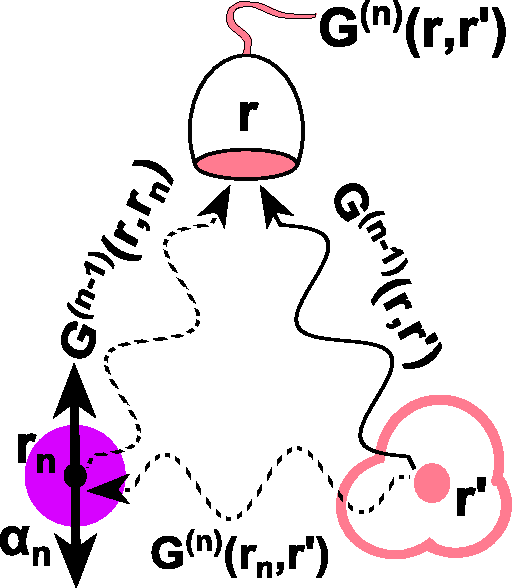
\includegraphics[width=5cm]{./Figs/GnDetection}%[bb=1.0in 1.0in 7.5in 10in]
\end{center}
\caption[The physics picture of Dyson equations.]{\textbf{The physics picture of the $n$-th order Dyson equations for $\Gn(\rr)$.} The solid wave illustrates the direct source emission path from $\br'$ to $\br$. The dashed wave illustrates the scattering path through the $n$-th dipole at $\br_n$. The cloud around $\br'$ illustrates that $(n-1)$ dipoles have been re-normalized as a single unit through the iteration of the $(n-1)$-th order of Dyson equations. }
\label{GnDetection}
\end{figure}

Instead of solving Equ.\eqref{dysonGN} directly, we can also adopt an iterative
scheme by rewriting a series of Dyson equations as
\begin{equation}
 \label{dysonGn}
\Gn(\rr)=\Gm1(\rr)+{\Gm1(\rrn)\cdot {\bm \alpha}_n \cdot \Gn(\mathbf{r}_n,\mathbf{r}')}.
\end{equation}
for $1 \leq  n \leq  N$. Equ. (\ref{dysonGn}) together with the symmetry relation
\begin{equation}
\label{symG2}
 G_{ji} \left(\br',\br,\omega\right) = G_{ij} \left(\br,\br',\omega\right)
\end{equation}
 forms the basis of GFTs and our calculation scheme in which QDs are
added to the system one by one in a self-consistent manner (see Fig.~\ref{GnDetection} for the physics picture). To solve this series of equations, as above, we also first place the detector at dipole positions. It gives interacting terms
\begin{equation}
\label{dysonGnij}
\Gn(\mathbf{r}_i,\mathbf{r}_j)=\Gm1(\mathbf{r}_i,\mathbf{r}_j)+{\Gm1(\mathbf{r}_i,\mathbf{r}_n)\cdot {\bm \alpha}_n\cdot \Gn(\mathbf{r}_n,\mathbf{r}_j)}.
\end{equation}
These interacting GFTs are first worked out for $\mathbf{r}_i=\mathbf{r}_n$, and this result is used to compute GFTs for $\mathbf{r}_i \neq \mathbf{r}_n$. As we increasing $n$ from 1 to $N$, we can solve the full Dyson equations in a straightforward iteration procedure based on bare cavity GFTs, which are supposed to be in Lorentzian forms as
\begin{equation}
 \label{Gcav}
\mathbf{G}^{(0)}(\br,\br',\omega)=\sum_{c}{\frac{\omega^2\mathbf{f}_{c}(\mathbf{r},\omega_{c})\mathbf{f}_{c}^*(\mathbf{r}',\omega_{c})}
{\omega_{c}^2-\omega^2-i\omega\Gamma_{c}}},
\end{equation}
with $c$ denoting modes of the cavity (we consider single mode case as default), $\omega_c$ the mode resonance, $\Gamma_{c}$ the decay rate or FWHM of $\mathbf{f}_{c}(\omega)$ for the corresponding mode.
For simplicity, all formulas below implicitly include the parameter $\omega$ unless explicitly stated otherwise.

Now, let's only consider 1-D case, which means all vectors and tensors are reduced to scalars. This truncation of dimensions is useful to study the optical properties of the cavity-QED system in one polarized direction. We particularly focus on the two simple scenarios, of which the GFs can be solved analytically without using a time-consuming iterative computation procedure.

\subsection{Two Analytical Scenarios}\label{section:scenarios}
In the following two sections, we will start to look at the spectrum of many photon emitters coupled with a single cavity mode, which has a relatively high Q or small non-radiative decay rate, $\Gamma_c$, and a well-defined intrinsic resonance, $\omega_0$. Notice that we define the observed cavity resonance at the peak position of the cavity spectrum as $\omega_c$, which gives $\omega_c \equiv \omega_0$ if there is no exciton coupled to the cavity. We regard every exciton as a dipole. The number of dipoles in a cavity system may not be the number of physical particles, such as QDs, since every particle can be excited to generate zero or many excitons~\footnote{Although excitons with the same resonance are forbidden to be at the same position by the exclusion principle, there can be several excitons with different resonances in a single quantum dot due to multi excited energy levels. One example of more than one exciton in a single elongated quantum dot was studied in Refs.~\cite{Muller2004,Gammon1996}. The existence of many excitons in the case of elongated QDs above is the consequence of shape anisotropy of the QDs.}. We suppose the background dipoles have the same amplitude of optical moments, $\bm{\mu}_n$, yet have different resonances of $\Omega_n$, where the subscript $n$ labels different background dipoles. In most of our discussions, we only look at the spectrum projected in one direction, and all vectors and tensors are reduced to scalars. The resonances of the background dipoles are randomly distributed according to the energy bands of the material, temperature~\cite{Li2005a,Wei2006}, sizes and shapes\cite{Imamoglu1999,Wang2007,Ratchford2011} of QDs, for example. Here, we used a Gaussian distributed dipole ensemble, which has a central resonance of $\Omega_d$ and a standard deviation of $\sigma$.

Below, we will mainly discuss two scenarios for the background dipoles. One is that all dipoles are located in a homogeneous field, with a unique coupling strength, $g_b=g_n=g$, defined by
\begin{equation}
g_{n}=\sqrt{\frac{\omega_c}{2\hbar \varepsilon_0}}\boldsymbol{\mu}_n\cdot \mathbf{f}_c(\mathbf{r}_n),
\end{equation}
where $\mathbf{f}_c(\mathbf{r}_n)=\mathbf{f}_c(\mathbf{r}_n,\omega_c)$ denotes the cavity mode or field strength at the $n$-th background dipole positioned at $\mathbf{r}_n$. In this case, we have assumed that the dot product of dipole moments and the on-site field is constant, and the amplitude of the field strength on the dipole oscillation direction is constant. This scenario is suitable for some micropillar, microdisk and similar devices, which have a smooth and near-homogeneous field strength for the emitting mode.

The other scenario is that there are a few primary or target emitting dipoles strongly excited with relatively large coupling strengths, $g_t$, and all the background dipoles share the same smaller coupling strength, $g_b=g$. To simplify the analysis, we will consider the case with only one target dipole. This scenario is usually suitable for photonic crystal cavities and similar cases which have one or several designed strong field spots to position target emitters. The target dipole will be labeled with subscript $t$.

To calculate the PL spectrum, the method developed by Wubs, Hughes and collaborators~\cite{Wubs2004,Kristensen2011,Wubs2012} was followed, which has been applied to one- and two-QDs coupled micropillar cavity and PC cavity systems\cite{Yao2009b,Yao2009c,Yao2009a,VanVlack2011,Reitzenstein2010,Hughes2009,Kristensen2011}. The key step to calculate the spectrum is to obtain the GFs including $N$ dipoles. Generally, the Green functions can be iteratively solved to obtain numerical values based on Dyson equations presented in the last sections~\cite{Wubs2004}, and cannot be written explicit analytical expressions. It is time- and memory-consuming to numerically calculate the GFs including a large number of dipoles. Fortunately, in the two scenarios we introduced above, one can obtain the analytical expressions of the Green function with any number of dipoles and complete the statistical analysis of collective emitting effects easily.

We present the main results of the Green functions for the two scenarios introduced above as follows. A detailed derivation can be found in the appendix~\ref{App:GF_ensemble}.

For scenario one, which does not have an identified target dipole, the Green functions including $n$-dipoles (labeled by $(n)$ in the superscripts) are
\begin{align}
\label{Gn11}
 G^{(n)}_{R_b,R_b}&=\frac{G^{(0)}_{R_b,R_b}}{1-G^{(0)}_{R_b,R_b}\sum_i^n{\alpha_i}},\\
\label{GnR1}
 G^{(n)}_{R,R_b}&=\frac{G^{(0)}_{R,R_b}}{1-G^{(0)}_{R_b,R_b}\sum_j^n{\alpha_j}}.
\end{align}
For short hand, we have labeled the first subscript of GFs as the detector,
and labeled the second subscript of GFs as the source.
That is to say, the subscripts of GFs defined in this section correspond to the arguments of detector and source positions in the normal GF definitions. For example, $G^{(n)}_{R,R_b}=G^{(n)}(R,R_b,\omega)$. Again, $\omega$ is implicit for all variables.

%Please notice that both equations ~\ref{Gn11} and ~\ref{GnR1} only have one cumulative variable, which is $\sum_j^n{\alpha_j}$, so to calculate the series of \{$G^{(n)}$\} that we can simply apply high-efficient matrix operators within a few steps by avoiding time-consuming iteration procedure in Matlab.



For scenario two, where there is one target dipole with a relatively large coupling strength and all the other background dipoles are in a mean weak field, the Green functions are
\begin{subequations}
\label{G1RR}
\begin{align}
 G^{(1)}_{R_t,R_j} &=\frac{G^{(0)}_{R_t,R_j}}{1-G^{(0)}_{R_t,R_t}\alpha_t},\quad j=t,b,\\
  G^{(1)}_{R,R_t} &=\frac{G^{(0)}_{R,R_t}}{1-G^{(0)}_{R_t,R_t}\alpha_t}, \\
  G^{(1)}_{R,R_b} &=G^{(0)}_{R,R_b}+\frac{G^{(0)}_{R,R_t}\alpha_t G^{(0)}_{R_t,R_b}}{1-G^{(0)}_{R_t,R_t}\alpha_t},\\
  G^{(1)}_{R_b,R_b} &=G^{(0)}_{R_b,R_b}+\frac{G^{(0)}_{R_b,R_t}\alpha_t G^{(0)}_{R_t,R_b}}{1-G^{(0)}_{R_t,R_t}\alpha_t},\label{G1RbRb}
\end{align}
\end{subequations}
and for $n\geq 1$
\begin{subequations}
\label{Gn+1RtRj}
\begin{align}
 G^{(n+1)}_{R_t,R_j} &=\frac{G^{(n)}_{R_t,R_j}}{1-G^{(n)}_{R_t,R_t}\alpha_t} \label{Gn+1RtRj1}\\
&= \frac{G^{(1)}_{R_t,R_j}}{1-G^{(1)}_{R_b,R_b}\sum_p^n{\alpha_p}},\quad j=b,t,\label{Gn+1RtRjexpand}
\end{align}
\end{subequations}
\begin{align}
  G^{(n+1)}_{R,R_b} &=\frac{G^{(1)}_{R,R_b}}{1-G^{(1)}_{R_b,R_b}\sum_i^n{\alpha_i}},\\
 G^{(n+1)}_{R,R_t} &=G^{(n)}_{R,R_t}+\frac{G^{(n)}_{R,R_b}\alpha_n G^{(n)}_{R_b,R_t}}{1-G^{(n)}_{R_b,R_b}\alpha_n}, \label{Gn+1RRt}\\
  G^{(n+1)}_{R_b,R_b} &=\frac{G^{(1)}_{R_b,R_b}}{1-G^{(1)}_{R_b,R_b}\sum_i^n{\alpha_i}}.\label{Gn+1RbRb}
\end{align}

Again, the equations above indicate that the Green functions including $N$ dipoles depend on the coupling term of all background dipoles. The difference between the two scenarios is that the target dipole changes the bare Green functions and hence the Green function including the target dipole plays a role as the bare Green functions do in scenario one. We would also like to keep Equs.\eqref{Gn+1RtRj1} and~\eqref{Gn+1RRt} in the iterative forms, which indicate the scattering effect from the $n$ background dipoles to the target dipole.

Also notice that the GFs of scenario one and scenario two are similar to one- and two-dipole coupled cavities, if comparing them with the formulas in, for example, Refs.~\onlinecite{Yao2009c,Kristensen2011}. The only difference is that the self energy term~\cite{Mahan2000}, $\sum_j^n{\alpha_j}$, replaces an individual $\alpha$, which is used for few-dipole cases. Therefore, the sum term indicates that the coupled background dipoles oscillate as an entity. Particularly, if all background dipoles share the same resonance and optical moment, it leads to
\begin{equation}
\sum_j^n{\alpha_j}=n\alpha,
\end{equation}
which means that, if we treat the ensemble as a single dipole, the effective optical moment and effective coupling strength are enlarged by $\sqrt{N}$ folds from the individual dipole. In this case, the GFs are simplified to
\begin{equation}
\label{equivGn11}
 G^{(n)}_{R_b,R_b}=\frac{G^{(0)}_{R_b,R_b}}{1-nG^{(0)}_{R_b,R_b}\alpha},
\end{equation}
\begin{equation}
\label{equivGnR1}
 G^{(n)}_{R,R_b}=\frac{G^{(0)}_{R,R_b}}{1-nG^{(0)}_{R_b,R_b}\alpha}.
\end{equation}

In general, $\alpha$ is a Lorentzian function of $\omega$; however, $\sum_j^n{\alpha_j}$ for an ensemble of dipoles may not be so. This fact leads to inhomogeneous broadening phenomena, as will be discussed in Chapter~\ref{ch:ensemble}. Moreover, scenario one is just a special case of scenario two when $g_t=g_b$.

Because of the clear physical picture and wide applicability, in Chapter~\ref{ch:ensemble}, we will mainly focus on the two scenarios mentioned above. The conclusions should be extendable to more general cases.

%{\textbf{Extension to Coupled-bin Model:}}
%Particularly, if we further make all excited resonant frequencies of QDs as the same value, which gives $\alpha_i=\alpha$, Equs.\eqref{Gn11} and ~\ref{GnR1} can be simplified into
%\begin{equation}
%\label{equivGn11}
% G^{(n)}_{R_b,R_b}=\frac{G^{(0)}_{R_b,R_b}}{1-nG^{(0)}_{R_b,R_b}\alpha},
%\end{equation}
%\begin{equation}
%\label{equivGnR1}
% G^{(n)}_{R,R_b}=\frac{G^{(0)}_{R,R_b}}{1-nG^{(0)}_{R_b,R_b}\alpha}.
%\end{equation}
%compared with first order Green's function and Equ.\eqref{alphanw}, we find that this ensemble is equivalent to one single QD with $\sqrt{n}$ times larger optical moment than real individual QD. And for general cases, ensemble properties cannot be generalized as easy as this particular case. However, if there are $N$ dots around one fixed frequency, their accumulated contribution to the total spectrum is not necessarily be their sum, and spectral amplitudes between two different frequencies also cannot be simply weighted by the corresponding numbers at those frequencies. Strictly speaking, this conclusion is contrast to reference \cite{meldrum2010} where the authors used homogeneous assumption. (More conclusions can be provided, if you are interested in.)

%In reality, researchers usually treat emitters with nearby resonances as one single dipole, or in most cases they can not distinguish individual excitons with close resonance. Equs.\eqref{equivGn11, equivGnR1} provide a theoretical origin of the equivalence between single dipole and many dipoles. Let's call it {\textit{coupled-bin}} model. However, as the cavity plays a role in the interaction, we should not use coupled-bin model or treat one QD as a single dipole any more in some cases. We will discuss it in the end of Chapter~\ref{ch:ensemble}.

\subsection{Incoherent Spectrum of an Ensemble Coupled Cavity}
One goal of calculating GFTs or GFs is to calculate the emission spectrum or field distribution in the presence of $N$ dipoles.
By definition, the emission power spectrum is given by
\begin{equation}
 \label{spectrumdef}
\begin{split}
S(\mathbf{r},\omega) =& \int_0^\infty \!\! \int_0^\infty\!\!
\mathrm{d}t_1\mathrm{d}t_2 \, e^{i\omega(t_2-t_1)}\mathinner{\langle}\hat{\mathbf{E}}^-(t_1)\hat{\mathbf{E}}^+(t_2)\mathinner{\rangle} \\
=& \mathinner{\langle} \left( \int_0^\infty \!\! \mathrm{d}t \, e^{i \omega t} \hat{\mathbf{E}}^+(t) \right)^{\dagger} \, \int_0^\infty \! \!
\mathrm{d}t \, e^{i\omega t} \hat{\mathbf{E}}^+(t) \mathinner{\rangle},
\end{split}
\end{equation}
where
\begin{equation}
 \label{eq:E^plus}
 \mathbf{\hat{E}}^+(\mathbf{r},t)
 =i\sum_\lambda\sqrt{\frac{\hbar\omega_\lambda}{2\varepsilon_0}}a_\lambda(t)\mathbf{f}_\lambda(\mathbf{r}).
\end{equation}
$a_\lambda$ is the annihilation operator for photons with angular frequency of $\omega_\lambda$.
Now,
\begin{align}
\int_0^\infty \! \mathrm{d} t \, e^{i\omega t} \hat{\mathbf{E}}^+(t) &= \int_0^\infty \! \mathrm{d}t \, e^{i\omega t}
\left[ \frac{1}{2\pi} \int_0^\infty \mathrm{d}\omega' \, e^{-i\omega' t} \mathbf{\hat{E}}(\omega')\right]  \nonumber\\
&= \frac{1}{2 \pi} \int_0^\infty \!\! \mathrm{d}\omega' \, \mathbf{\hat{E}}(\omega') \int_0^\infty \!\! \mathrm{d}t \, e^{i(\omega-\omega') t} \nonumber\\
&= \frac{1}{2\pi} \int_0^\infty \! \mathrm{d}\omega' \, \mathbf{E}(\omega')\left[iP(\frac{1}{\omega-\omega'})+\pi\delta(\omega-\omega')\right] \label{specP} \\
&= \frac{1}{2\pi}\pi(\mathbf{\hat{E}}(\omega)+\mathbf{\hat{E}}(\omega))\nonumber\\
&= \mathbf{\hat{E}}(\omega),
\end{align}
where $ P $ is the principle value function~\cite{Carmichael2007}, and Cauchy's integral formula\footnote{See Ref.~\cite{VanVlack2012} for details.} has been used to give $P[1/(\omega-\omega')]=-i\pi$.
The power spectrum can be simply expressed (see also \cite{Hughes2009})
\begin{equation}\label{eq:spectrum}
 S({\bf r},\omega)=\langle
(\mathbf{\hat{E}}(\omega))^{\dagger}\mathbf{\hat{E}}(\omega)\rangle.
\end{equation}
Notice that this is a non-Markovian solution, valid for any spatial position $\mathbf{r}$.

Once the power spectrum or photoluminescence (PL) spectrum is obtained in the frequency domain, it is easy to get the luminescence dynamic curve in the time domain,
merely by performing a Fourier transformation.

From Equ.\eqref{E4GNS_1}, we can get the incoherent spectrum formula for the $N$-dipole coupled cavity system as
\begin{equation}
 \label{spectrum}
 \mathbf{S}(\br,\omega)=\left|\mathbf{E}^{(N)}(\br,\omega)\right|^2,
\end{equation}
where
\begin{equation}
 \left| \mathbf{E}^{(N)}(\br,\omega)\right| =\frac{1}{\varepsilon_0}\langle \sum_n{\GN(\rrn,\omega)\cdot \dnw}\rangle.
\end{equation}

We will discuss the spectra of several cases under the single excitation approximation in the following subsections. At the end of this section,
we will define a proper initial condition for the $N$-dipole coupled cavity,
to be discussed in the next chapters.
%In equations above, subscription ``c'' means cavity term which includes the bare cavity field and scattering term; the subscription ``s'' means source term, which is the contribution from all photon emitters.

Below, we will discuss the initial conditions and spectrum calculations for several cases. As will be shown, to analyze the spectrum of optical cavities with $N$ dipoles, the roadmap that we first calculate the total GFTs including any $n\,(n\leq N)$ dipoles and then calculate the corresponding spectra is feasible and efficient for spectral analysis; the mixed state with equally excited dipoles under the single excitation condition is a good initial condition for our calculation, both because of its simplicity and its representativeness for practical cases. At the end of this section, we will obtain the general spectral formula for the $N$ dipoles coupled cavity under the mixed state initial condition.
\subsubsection{Case 1: One-dipole system initially with one exciton and no photon}

We assume an initially excited dipole at ${\bf r}'={\bf r}_1$,
so that we can write the initial
condition as
$\ket {\Psi(t=0)}=\ket{0}_{\rm c}\ket 1_{\rm x}=\sigp\ket{0}$, where the ket with subscript $x$ indicates whether the dipole is excited, and the ket with subscript $c$ indicates the photon number in the cavity. The ket $\ket{0}$ is the ground state of $\ket{0}_c\ket{0}_x$.

For a one-dipole system, Equ.\eqref{E4GNS} gives the exact electric field operator responding at $\br$ as
\begin{equation}
\mathbf{\hat{E}}^{(1)}(\mathbf{r},\omega)=\frac{1}{\varepsilon_0}\mathbf{G}^{(0)}(\mathbf{r},\mathbf{r}_1,\omega)\cdot
{\bf
e}_1\hat{d}_1(\omega)+\mathbf{G}^{(0)}(\mathbf{r},\mathbf{r}_1,\omega)\cdot
{\bf e}_1 \alpha_1(\omega) \hat{E}^{(1)} (\mathbf{r}_1,\omega),
\end{equation}
%\begin{equation}
%\hat{\mathbf{E}}^{(1)}(\mathbf{r},\omega) ={\mathbf{G}^{(0)}(\br,\br_1,\omega)\cdot \hat{\mathbf{d}}_1(\omega)}
%  +{\mathbf{G}^{(0)}(\br,\br_1,\omega)\cdot {\bm \alpha}_1(\omega) \cdot \hat{\mathbf{E}}^{(1)}(\mathbf{r}_1,\omega)}
%\end{equation}
where we have assumed the initial E-field strength at the detector position to be zero, or $\E0=0$ with ${\bf r}\neq {\bf r}_1$. This condition is a requirement of our GF method, as have been assumed in Equ.\eqref{eq:EGP}.

%\begin{equation}
%\hat{\mathbf{E}}^{(1)}
%(\mathbf{r}_1,\omega)=[\eye-
%\mathbf{G}^{(0)}(\mathbf{r}_1,\mathbf{r}_1,\omega)\cdot
%\, {\bm \alpha}_1(\omega)]^{-1}\cdot{
%\mathbf{G}^{(0)}(\mathbf{r}_1,\mathbf{r}_1,\omega)\cdot
%\hat{\mathbf{d}}_1(\omega)}.
%\end{equation}
%\begin{eqnarray}
%\mathbf{\hat{E}}^1(\mathbf{r},\omega)=\mathbf{G}^{(0)}(\mathbf{r},\mathbf{r}_1,\omega)\cdot
%{\bf
%e}_1\hat{d}_1(\omega)+\mathbf{G}^{(0)}(\mathbf{r},\mathbf{r}_1,\omega)\cdot
%{\bf e}_1 \alpha_1(\omega) \hat{E}^1 (\mathbf{r}_1,\omega).
%\end{eqnarray}
The E-field at $\br_1$ can be obtained from Equ.\eqref{E4GNS_0} by setting $N=0$ and ${\bf r}= {\bf r}_1$. The projection of $\mathbf{\hat{E}}^{(1)}(\mathbf{r},\omega)$ in ${\bf e}_1$ is given by\footnote{see Appendix~\ref{section:GFscalar} for details.}
\begin{equation}\label{E1projection}
\hat{E}^{(1)}
(\mathbf{r}_1,\omega)=\mathbf{\hat{E}}^{(1)}(\mathbf{r}_1,\omega)\cdot{\bf e}_1=\frac{1}{\varepsilon_0}\frac{{\bf e}_1
\cdot\mathbf{G}^0(\mathbf{r}_1,\mathbf{r}_1,\omega)\cdot
\mathbf{e}_1 \, \hat{d}_1(\omega)}{[1-{\bf e}_1
\cdot\mathbf{G}^0(\mathbf{r}_1,\mathbf{r}_1,\omega)\cdot {\bf e}_1
\, \alpha_1(\omega)]}.
\end{equation}
Using Equ.\eqref{E4GNS_1}, one can obtain
\begin{equation}
\mathbf{\hat{E}}^{(1)}(\mathbf{r},\omega)=\frac{1}{\varepsilon_0}\frac{\mathbf{G}^{(0)}(\mathbf{r},\mathbf{r}_1,\omega)\cdot
\mathbf{e}_1 \, \hat d_1(\omega)}{[1-{\bf e}_1
\cdot\mathbf{G}^{(0)}(\mathbf{r}_1,\mathbf{r}_1)\cdot {\bf
e}_1\,\alpha_1(\omega)]}
=\frac{1}{\varepsilon_0}\mathbf{G}^{(1)}(\mathbf{r},\mathbf{r}_1,\omega)\cdot
{\bf e}_1 \, \hat{d}_1(\omega),
\end{equation}
where $\mathbf{G}^{(1)}(\mathbf{r},\mathbf{r}_1,\omega)=\mathbf{G}^{1}_1(\mathbf{r},\mathbf{r}_1,\omega)$ indicates the ``renormalized''
GF including the one dipole's contribution~\footnote{$\mathbf{G}^{1}_1(\mathbf{r},\mathbf{r}_1,\omega)$ is defined by Equ.\eqref{Gi1}.}. Note that $\br$ is implicitly included in the E-field operators below.
Now,
\begin{align}
\mathbf{\hat{E}}^{(1)}(\omega)\ket {\Psi(t=0)}&=
\frac{i}{\varepsilon_0}\mathbf{G}^{(1)}(\mathbf{r},\mathbf{r}_1,\omega)\cdot
{\bm \mu_1} \left [
\frac{\hat{\sigma}^-(t=0)}{\omega-\Omega_1}+\frac{\hat{\sigma}^+(t=0)}
{\omega+\Omega_1}\right ] \ket{0}_c\ket{1}_x
\nonumber \\
&=\frac{i}{\varepsilon_0}\mathbf{G}^{(1)}(\mathbf{r},\mathbf{r}_1,\omega)\cdot
{\bm \mu_1}
\frac{1}{\omega-\Omega_1}\ket{0}.
\end{align}
%where we have defined $\ket{0}=\ket{0}_c\ket{0}_x$.
The spectrum is therefore
\begin{align}
\braket{(\mathbf{\hat{E}}^{(1)}(\omega))^\dagger\mathbf{\hat{E}}^{(1)}(\omega)}
&=\bra{\Psi(t=0)}(\mathbf{\hat{E}}^{(1)}(\omega))^+ \mathbf{\hat{E}}^{(1)}(\omega)\ket {\Psi(t=0)} \nonumber\\
%&=
%\frac{1}{\varepsilon_0^2}|\mathbf{G}^{(1)}(\mathbf{r},\mathbf{r}_1,\omega)\cdot
%{\bm \mu_1}|^2 \bra{0}\left [\sigm \left|
%\frac{\hat{\sigma}^-(t=0)}{\omega-\Omega_1}+\frac{\hat{\sigma}^+(t=0)}
%{\omega+\Omega_1}\right| ^2 \sigp\right ]\ket{0}
%\nonumber \\
%&=\frac{1}{\varepsilon_0^2}|\mathbf{G}^{(1)}(\mathbf{r},\mathbf{r}_1,\omega)\cdot
%{\bm\mu_1}|^2 \bra{0}
%[\frac{\sigm\sigm\sigp\sigp}{(\omega+\Omega_1)^2}
%+\frac{\sigm\sigp\sigm\sigp}{(\omega-\Omega_1)^2}\nonumber\\
%&\quad \quad \quad \quad \quad \quad
%+\frac{\sigm\sigp\sigp\sigp}{\omega^2-\Omega_1^2}
%+\frac{\sigm\sigm\sigm\sigp}{\omega^2-\Omega_1^2}]\ket{0} \nonumber\\
&= \frac{1}{\varepsilon_0^2}|\mathbf{G}^{(1)}(\mathbf{r},\mathbf{r}_1,\omega)\cdot
{\bm\mu_1}|^2 \frac{1}{|\omega-\Omega_1|^2}.
\end{align}
Considering the decay rate from the dipole (see footnote~\ref{fn:decayrevision}), we finally have
\begin{align}
S({\bf r},\omega) &= \braket{(\mathbf{\hat{E}}^{(1)}(\omega))^\dagger\mathbf{\hat{E}}^{(1)}(\omega)} \nonumber \\ &= \frac{1}{\varepsilon_0^2} |\mathbf{G}^{(1)}(\mathbf{r},\mathbf{r}_1,\omega)\cdot
{\bm\mu_1}|^2 \frac{1}{|\omega-\Omega_1+i\Gamma_1/2|^2}.\label{eq:spec_1dipole}
\end{align}
The equation above shows that the spectrum has two peaks: one is close to the cavity resonance, implicitly indicated by the denominator of $\mathbf{G}^{(1)}(\mathbf{r},\mathbf{r}_1,\omega)$; the other is at the dipole resonance,
indicated by the denominator $|\omega-\Omega_1+i\Gamma_1/2|^2$.
Besides, the spectrum function is a combination of Lorentzian functions.
%
%Rewriting the denominator as
%$\omega^2-\Omega_1^2-\omega\Sigma(\omega)$, with $\Sigma(\omega)$
%the usual self-energy, we see that the radiative decay is given by
%${\rm Im}[\Sigma(\Omega_1)]=2\hbar^{-1} \varepsilon_0^{-1}\mu_1^2
%{\rm Im}\,[{\bf K}({\bf r}_1,{\rm r}_1;\Omega_1)]$, which agrees
%perfectly with other derivations of the radiative decay in general
%media, e.g by Welsch and co-workers~\cite{Dung2000}, who
%typically formulate in terms of ${\bf G}$--note that we have ${\rm
%Im}\,[{\bf K}]={\rm Im}\,[{\bf G}]$, which is true for lossless
%media, namely real $\varepsilon({\bf r})$.
%
%It should also be noted that the above expression fully recovers
%weak to strong coupling in a self-consistent way, so this
%definition of radiative decay assumes weak coupling. Checking for
%a homogeneous medium, where here ${\rm Im}[{\bf
%K}(\Omega_1)]=\Omega_1^3\sqrt{\varepsilon}/(6\pi c^3)$, then this
%recovers the well known Einstein `A' coefficient, namely
%$\Gamma_{\rm A}=\Omega_1^3\mu_1^2\sqrt{\varepsilon}/(3\hbar\varepsilon_0c^3)$.\\

\subsubsection{Case 2: One-dipole system initially with one photon and no exciton}
In the case that there is only one photon in the cavity while the only dipole is in the ground state, the initial condition can be written as
$\ket{\Psi(t=0)}= \ket{1}_{c} \ket 0_{\rm x}=a^{\dagger}_c\ket{0}$. Here, we have assumed that only one mode has dominated the cavity field, $\mathbf{f}_c(\mathbf{r})$, and $\adag_c=a^{\dagger}_c(t=0)$ is the creation operator to generate a photon with the angular frequency of $\omega_c$ in the cavity. We also assume that the detector is far from the photon source ($r\rightarrow \infty$), which is the case of the far field measurement coveries most of our discussions, and the initial condition of $\mathbf{\hat{E}}^{(0)}(\mathbf{r},\omega)=0$ holds to give the formula of $\hat{E}^{(1)}(\mathbf{r}_1,\omega)$ in Equ.\eqref{E1projection}. Adapting Equ.\eqref{eq:E^plus} at the dipole, one can assume the initial E-field gives
$$\mathbf{\hat{E}}^{(0)}(\mathbf{r}_1,\omega)
 =-\sqrt{\frac{\hbar\omega_c}{2\varepsilon_0}}a_c(t=0)\mathbf{f}_c(\mathbf{r}_1) /(\omega-\omega_c)$$
In the equation above, we have assumed a lossless cavity mode. We will include the cavity decay rate, $\Gamma_c$,
in the final spectrum formula as we did in the last case.
%
The electric field operator is now
\begin{equation}
\mathbf{\hat{E}}^{(1)}({\bf
r},\omega)=\mathbf{G}^{(0)}(\mathbf{r},\mathbf{r}_1,\omega)\cdot
{\bm \alpha}_1(\omega) \hat{E}^{(1)}(\mathbf{r}_1,\omega).
\end{equation}
%Note that we have explicitly included the $\mathbf{\hat{E}}^{(0)}(\mathbf{r},\omega)$ term.
Hence one has
\begin{align}
\mathbf{\hat{E}}^{(1)}({\bf
r},\omega)&=\mathbf{G}^{(0)}(\mathbf{r},\mathbf{r}_1,\omega)\cdot \mathbf{e}_1
\alpha_1(\omega) \frac{{\bf e}_1 \cdot\hat{{\bf E}}^{(0)}({\bf r}_1,\omega)}
{1-{\bf e}_1 \cdot {\bf G}^{(0)}({\bf r}_1, {\bf r}_1, \omega) \cdot
{\bf e}_1 \alpha_1(\omega)}\\
&=\mathbf{G}^{(1)}(\mathbf{r},\mathbf{r}_1,\omega)\cdot {\bm \alpha}_1(\omega) \cdot \hat{{\bf E}}^{(0)}({\bf r}_1,\omega).
\end{align}

Projecting into the initial ket state, the E-field operator leads to
\begin{align}
\!\!\!\!\!\!\!\!\! &\quad\mathbf{\hat{E}}^{(1)}({\bf r},\omega)\ket{\Psi(t=0)}\nonumber \\
&= \mathbf{\hat{E}}^{(1)}({\bf r},\omega)
 a^{\dagger}_c(t=0)\ket{0}_{c}\! \ket 0_{\rm x}\nonumber\\
&= -\sqrt{\frac{\hbar
\omega_c}{2\varepsilon_0}}\left [
\mathbf{G}^{(1)}(\mathbf{r},\mathbf{r}_1,\omega)\cdot {\bm \alpha}_1(\omega) \cdot \!
\mathbf{f}_c(\mathbf{r}_1) \! \right]\!
\frac{a_c a^{\dagger}_c(t\!=\!0)}{\omega-\omega_c}\ket
{0}_{c}\!\ket 0_{\rm x}\nonumber\\
%&= -\sqrt{\frac{\hbar
%\omega_\lambda}{2\varepsilon_0}}\left [
%\mathbf{G}^{(1)}(\mathbf{r},\mathbf{r}_1,\omega)\cdot {\bm \alpha}_1(\omega) \cdot \!
%\mathbf{f}_c(\mathbf{r}_1) \! \right]\frac{1}{\omega-\omega_c} \ket{0}\nonumber\\
&= \sqrt{\frac{\hbar
\omega_c}{2\varepsilon_0}}\left [\mathbf{G}^{(1)}(\mathbf{r},\mathbf{r}_1,\omega)\cdot {\bm \alpha}_1(\omega) \cdot \!
\mathbf{f}_c(\mathbf{r}_1) \! \right]\frac{1}{\omega_c-\omega}\ket{0},
\end{align}
and so
\begin{align}
S({\bf r},\omega)&= \bra{\Psi(t=0)}\left(\mathbf{\hat{E}}^{(1)}({\bf
r},\omega)\right)^\dagger \mathbf{\hat{E}}^{(1)}({\bf
r},\omega)\ket{\Psi(t=0)}  \nonumber\\
&= \left |\sqrt{\frac{\hbar
\omega_c}{2\varepsilon_0}}\left [
\mathbf{G}^{(1)}(\mathbf{r},\mathbf{r}_1,\omega)\cdot {\bm \alpha}_1(\omega) \cdot \!
\mathbf{f}_c(\mathbf{r}_1) \!\right
]\right
|^2\frac{\bra{0}a_c \adag_c a_c \adag_c\ket{0}}{(\omega-\omega_c)^2}\nonumber \\
&= \left |\sqrt{\frac{\hbar
\omega_c}{2\varepsilon_0}}\left [
\mathbf{G}^{(1)}(\mathbf{r},\mathbf{r}_1,\omega)\cdot {\bm \alpha}_1(\omega) \cdot \!
\mathbf{f}_c(\mathbf{r}_1) \!\right
]\right
|^2\frac{\bra{0}a_c (a_c\adag_c -1) \adag_c\ket{0}}{(\omega-\omega_c)^2}\nonumber\\
&= \left |\sqrt{\frac{\hbar
\omega_c}{2\varepsilon_0}}\left [
\mathbf{G}^{(1)}(\mathbf{r},\mathbf{r}_1,\omega)\cdot {\bm \alpha}_1(\omega) \cdot \!
\mathbf{f}_c(\mathbf{r}_1) \!\right
]\right
|^2\frac{\bra{0}(a_c a_c\adag_c \adag_c-a_c\adag_c)\ket{0}}{(\omega-\omega_c)^2}\nonumber\\
&= \left |\sqrt{\frac{\hbar
\omega_c}{2\varepsilon_0}}\left [
\mathbf{G}^{(1)}(\mathbf{r},\mathbf{r}_1,\omega)\cdot {\bm \alpha}_1(\omega) \cdot \!
\mathbf{f}_c(\mathbf{r}_1) \!\right
]\right
|^2\frac{1}{(\omega-\omega_c)^2},\label{eq:s_init_f_0}
\end{align}
where I have used the commutator $[a_c, \adag_c]=1$.
%Since $\omega$ and $\omega_c$ are usually close to each other, one can use $(\omega-\omega_c)^2\approx |\omega^2-\omega_c^2|$.
Considering the revision of cavity decay rate, $\Gamma_c$, we can obtain the spectrum as
\begin{equation}
S({\bf r},\omega)=\left |\sqrt{\frac{\hbar
\omega_c}{2\varepsilon_0}}\left [
\mathbf{G}^{(1)}(\mathbf{r},\mathbf{r}_1,\omega)\cdot {\bm \alpha}_1(\omega) \cdot \!
\mathbf{f}_c(\mathbf{r}_1) \!\right
]\right
|^2\frac{1}{|\omega-\omega_c+i\Gamma_c/2|^2},\label{eq:s_init_f}
\end{equation}
Compared with the spectrum of the one-exciton case (Equ.\eqref{eq:spec_1dipole}), the spectrum of the one-photon case also has two peaks characterized by the dipole and cavity resonances, and is a combination of Lorentzian functions.
%; the main difference is that the two spectra may have different amplitudes at the same resonant peaks.
In the cases of the PC cavity studied in Chapter~\ref{ch:cavity}, the one-photon spectrum has a much larger amplitude yet quite similar lineshape compared with the one-exciton spectrum. The spectral form obtained via the GF method is quite general for an arbitrary initial field, as the field has been included in the $\mathbf{f}_c(\mathbf{r}_1)$ factor and bare cavity GFs.

The spectral calculation method discussed in cases 1\&2 has been applied to various one-dipole systems, including PC cavities and waveguides~\cite{Yao2009a,Yao2009b,Yao2009}. In the general case of one-dipole cavities, a geometrical factor $F(\br)$ is used in Ref.~\cite{Yao2009c} to adjust the scale under arbitrary initial conditions. Note that we always suppose there is no initial field at the detector position. In some cases such as a persisting oscillated waveguide, this condition may break, and the initial field strength at the detection position should be taken into account, which leads to
\begin{equation}\label{eq:longoscillatedwaveguide}
S({\bf r},\omega)= \left |\sqrt{\frac{\hbar
\omega_c}{2\varepsilon_0}}\left [\mathbf{f}_c(\mathbf{r})+
\mathbf{G}^{(1)}(\mathbf{r},\mathbf{r}_1,\omega)\cdot {\bm \alpha}_1(\omega) \cdot \!
\mathbf{f}_c(\mathbf{r}_1) \!\right
]\right|^2\frac{1}{|\omega-\omega_c+i\Gamma_c/2|^2}
\end{equation}
under the one-photon initial condition. However, considering the definition of the bare cavity GF in Equ.\eqref{eq:EGP}, Equ.\eqref{eq:longoscillatedwaveguide} is valid unless one modifies the bare cavity GFTs properly.

In cases 1\&2, we obtained the E-field operator before calculating the spectrum. This approach is straightforward in few-dipole coupled cavity cases. However, this approach may not work to obtain the spectrum of many-dipole coupled cavities. This is because a large-size matrix has to be inverted to obtain the E-field operator expressions at individual dipoles, and it is difficult to invert a matrix with a large size using limited computational resources (see Appendix~\ref{App:GF}). In the calculations below, we will use the equivalent equation of the total E-field at $\br$ (Equ.\eqref{E4GNS_1}), where we first calculate the GFTs with $n\,(n\leq N)$ dipoles and then calculate the target spectra responding at the detection position, to avoid the calculation of the total E-field from all the individual dipoles' positions.  At the end of this section, we will show the equivalence of these two roadmaps when $N=1$. One extra benefit of our approach is that we can easily obtain arbitrary $n\,(n\leq N)$ coupled spectrum as the GFTs is iterated from $n=0$ to $n=N$. This feature is efficient for the spectral analysis on various dipole numbers. Another benefit of our approach used below is that we can avoid the scale issue with the initial condition associated with photon excitations.

We will discuss some general initial conditions in the following two subsections; in Chapter~\ref{ch:cavity}, we will compare our calculation results of one- and two-dipole systems with already published results.



%However, a typical application would likely have no homogeneous
%field at the detector and an excited cavity mode photon; thus
%${\hat {\bf E}}_0({\bf r},\omega)=0$ ($\rightarrow{\bf f}_c({\bf
%r})=0$) and ${\hat {\bf E}}_0({\bf r}_1,\omega)=
%-\sqrt{\hbar\omega_c/2\varepsilon_0}\, {\bf f}_c({\bf r}_1) \hat
%a_c^0(\omega)/(\omega-\omega_c-i\Gamma_{c}/2)$~\cite{Reitzenstein2010}. With a strongly
%coupled QD, the spectral lineshape can look substantially
%different to the case of an excited QD in vacuum, as is obvious
%from the appearance of cavity lineshape in the spectrum. The
%spectrum now takes the form:
%
%\begin{eqnarray}
%S({\bf r},\omega)&=&\left | \sqrt{\frac{\hbar
%\omega_c}{2\varepsilon_0}}\left (
% \frac{\mathbf{K}(\mathbf{r},\mathbf{r}_1;\omega)\cdot
%{\bf n}_1 \alpha_1(\omega) {\bf n}_1 \cdot
%\mathbf{f}_\lambda(\mathbf{r}_1) }{1-{\bf n}_1 \cdot {\bf
%K}_c({\bf r}_1, {\bf r}_1, \omega)\cdot {\bf n}_1
%\alpha_1(\omega)}\right
%)\frac{1}{\omega_c-\omega+i\Gamma_c/2}\right |^2,
%\end{eqnarray}
%where the cavity Green function  ${\bf K}_c({\bf r}_1,{\bf
%r}_1;\omega) \approx \omega^2{\bf f}_c({\bf r}_1) {\bf
%f}_{c}^*({\bf r}_1) /(\omega^2-\omega_c^2+i\omega\Gamma_c)$.
%

%Another example is waveguide-single-cavity system and  have a
%photonic crystal waveguide mode, as the (quantum) {\em
%homogeneous} driving field ${\bf E}_{0}({\bf
%r,\omega})=[a/L]^{1/2}\, \tilde{\bf f}_{k_0}({\bf r})e^{ik_{0}x}$,
%with $\int_{\rm cell} \varepsilon({\bf r}) \tilde{\bf
%f}_{k_0}^*({\bf r}) \tilde{\bf f}_{k_0} ({\bf r})=1$ and $a$ is
%the pitch. Eq(\ref{eq:s_init_f})  assume the system has been
%stable and oscillated harmonically before adding quantum dot, so
%the initial field would be
%$\mathbf{E}(\mathbf{r},\omega)=\mathbf{E}_0(\mathbf{r},\omega)+\int
%d\mathbf{r}'\mathbf{K}(\mathbf{r},\mathbf{r}',\omega)V(\mathbf{r}')\mathbf{E}_0(\mathbf{r}',\omega)$.
%Here, we are  interested in $r\rightarrow \infty$,  only waveguide
%modes have contribution to the $S(\omega)$. The summation over
%$\lambda$ in Eq(\ref{eq:s_init_f}) can be changed into integral
%over $\bf k$. Then we have
%\begin{eqnarray}
%S({\bf r},\omega)_{\bf r \rightarrow \infty}&=&\left
%|\sqrt{\frac{\hbar \omega}{2\varepsilon_0}}\left [
%\mathbf{f}(\mathbf{r},\omega)+ \frac{
%\mathbf{K}(\mathbf{r},\mathbf{r}_1;\omega)\cdot {\bf n}_1
%\alpha_1(\omega)\, {\bf n}_1 \cdot \mathbf{f}(\mathbf{r}_1,\omega)
%}{1-{\bf n}_1 \cdot {\bf K}({\bf r}_1, {\bf r}_1;\omega)\cdot {\bf
%n}_1 \alpha_1(\omega)}\right ]\frac{C(\omega)\sqrt{2\pi
%L}}{v_g(\omega)}\right |^2.
%\end{eqnarray}
%
%Here, $C(\omega)$ is of the dimension of $\sqrt{L}$ and $\int
%|C|^2dk=1$. Notice that
%$\mathbf{K}(\mathbf{r},\mathbf{r}_1;\omega)$ in the numerator is
%dominated by $\ket {\mathbf{E}_k}\bra{\mathbf{E}_c}$ and
%$\mathbf{K}(\mathbf{r}_1,\mathbf{r}_1;\omega)$ is dominated by
%$\ket {\mathbf{E}_c}\bra{\mathbf{E}_c}$, we have
%$\mathbf{K}(\mathbf{r},\mathbf{r}_1;\omega)\approx{iL\omega^3}{\bf
%f}_{k_0}({\bf r}){\bf f}_c({\bf r}_1)\int d \mathbf{r}'{\bf
%f}_{k_0}^*({\bf r'})V(\mathbf{r}'){\bf f}_c({\bf
%r}')/({v_g(\omega^2-\omega_c^2+i\omega\Gamma_c)})$ and ${\bf
%K}({\bf r}_1,{\bf r}_1;\omega) \approx \omega^2{\bf f}_c({\bf
%r}_1) {\bf f}_{c}^*({\bf r}_1)
%/(\omega^2-\omega_c^2+i\omega\Gamma_c)$.Substitute
%$\mathbf{E}(\mathbf{r},\omega)=\mathbf{E}_0(\mathbf{r},\omega)+\int\mathbf{K}(\mathbf{r},\mathbf{r}',\omega)V(\mathbf{r}')\mathbf{E}_0(\mathbf{r}',\omega)d
%\mathbf{r}'=\mathbf{f}(\mathbf{r},\omega)$
% into the above equation. After renormalization, we can get the transmission
%\begin{eqnarray}
%T({\bf r},\omega)_{\bf r \rightarrow \infty}&=&\left |1+
%\frac{i\omega
%\Gamma_c}{(\omega^2-\omega_c^2+i\omega\Gamma_c-\omega^2{\bf
%f}_c({\bf r}_1) {\bf f}_{c}^*({\bf r}_1)\alpha_1 )}\right|^2
%\end{eqnarray}

\subsubsection{Case 3: Two-dipole system with equally excited dipoles}
In this section, we discuss two-dipole coupled cavities, where both dipoles have the same chance to be excited. We assume that there is no photon initially in the cavity or at the detection position, and on average there is only one exciton created in the cavity. One case of an equally excited dipole pair is that these two dipoles are in an entangled state $\ket{\Psi(t=0)}=b_1\ket{1}_1\ket{0}_2 + b_2\ket{0}_1\ket{1}_2 =b_1\ket{10} + b_2\ket{01} = (b_1\sigp_1+b_2\sigp_2)\ket{0}$, where we have made $\ket{ij}=\ket{i}_1\ket{j}_2$ to indicate the joint state of dipole 1 and dipole 2 ({\it i.e.} $\ket{10}$ means dipole 1 is excited while dipole 2 is in the ground state.); $\ket{0}=\ket{00}$. $\sigp_i$ is the creation operator for the $i$th exciton. $b_1$ and $b_2$ are the normalized coefficients to indicate the probability of the dipoles being in $\ket{10}$ or $\ket{01}$ states. For equally excited dipoles, we can make $b_1=b_2=1/\sqrt{2}$ under the normalized condition $|b_1|^2+|b_2|^2=1$. The cavity field state of $\ket{0}_c$ is implicitly included in the $\ket{\Psi(t=0)}$ state. If we let $\hat{n}_2=\sum_i{\sigp_i\sigm_i}$ be the number operator of excitons, we will find that $\braket{\hat{n}_2}=|b_1|^2+|b_2|^2=1$ which satisfies the condition of single excitation.

Equ.\eqref{E4GNS_1} leads to
\begin{equation}
\mathbf{\hat{E}}^{(2)}({\bf r},\omega) =\frac{1}{\varepsilon_0}[\mathbf{G}^{(2)}(\br,\br_1,\omega)\cdot \hat{\mathbf{d}}_1(\omega) + \mathbf{G}^{(2)}(\br,\br_2,\omega)\cdot \hat{\mathbf{d}}_2(\omega)].
\end{equation}
We let $C_i=\frac{i}{\varepsilon_0}\mathbf{G}^{(2)}(\br,\br_i,\omega)\cdot {\bm \mu}_i,\,\, i=1,2$, hence
\begin{align}
\!\!\!\! &\quad \mathbf{\hat{E}}^{(2)}({\bf r},\omega)\ket{\Psi(t=0)} \nonumber \\ &=\frac{1}{\varepsilon_0}[\mathbf{G}^{(2)}(\br,\br_1,\omega)\cdot \hat{\mathbf{d}}_1(\omega) + \mathbf{G}^{(2)}(\br,\br_2,\omega)\cdot \hat{\mathbf{d}}_2(\omega)](b_1\ket{10}+b_2\ket{01})\nonumber \nonumber \\
&= \left[C_1 \left( \frac{\sigm_1}{\omega-\Omega_1} \! + \! \frac{\sigp_1}{\omega + \Omega_1}\right) \! + \! C_2\left( \frac{\sigm_2}{\omega-\Omega_2} \! + \! \frac{\sigp_2}{\omega + \Omega_2} \right) \right](b_1\ket{10}+b_2\ket{01}) \nonumber \\
&= C_1\left( \frac{b_1\ket{00}}{\omega-\Omega_1} + \frac{b_2\ket{11}}{\omega + \Omega_1}\right) + C_2\left( \frac{b_2\ket{00}}{\omega-\Omega_2} + \frac{b_1\ket{11}}{\omega + \Omega_2} \right)\\
&= \left( \frac{C_1 b_2}{\omega+\Omega_1}+ \frac{C_2 b_1}{\omega+\Omega_2} \right)\ket{11} + \left( \frac{C_1 b_1}{\omega-\Omega_1}+ \frac{C_2 b_2}{\omega-\Omega_2} \right)\ket{00}\\
&= \frac{1}{\sqrt{2}}\left( \frac{C_1}{\omega+\Omega_1}+ \frac{C_2 }{\omega+\Omega_2} \right)\ket{11} + \frac{1}{\sqrt{2}} \left( \frac{C_1}{\omega-\Omega_1}+ \frac{C_2}{\omega-\Omega_2} \right)\ket{00}.
\end{align}
Consequently, the spectrum is given by
\begin{align}
&\quad S({\bf r},\omega) = \bra{\Psi(t=0)}\left(\mathbf{\hat{E}}^{(2)}({\bf
r},\omega)\right)^\dagger \mathbf{\hat{E}}^{(2)}({\bf
r},\omega)\ket{\Psi(t=0)}  \nonumber\\
&= \frac{1}{2}\bra{11}\left[ (\frac{C_1^*}{\omega+\Omega_1}+ \frac{C_2^*}{\omega+\Omega_2}) (\frac{C_1}{\omega+\Omega_1} + \frac{C_2}{\omega+\Omega_2}) \right]\ket{11} \nonumber \\
&\quad \quad \quad \quad \quad \quad \quad
+\frac{1}{2}\bra{00} \left[ (\frac{C_1^*}{\omega-\Omega_1}+ \frac{C_2^*}{\omega-\Omega_2})(\frac{C_1}{\omega-\Omega_1} + \frac{C_2}{\omega-\Omega_2}) \right]\ket{00} \nonumber \\
%&=  \frac{1}{2}\left[ \frac{|C_1|^2}{(\omega+\Omega_1)^2} + \frac{|C_2|^2}{(\omega+\Omega_2)^2} + \frac{C_1^*C_2+C_1C_2^*}{(\omega+\Omega_1)(\omega+\Omega_2)} \right] \nonumber \\
%&\quad \quad + \frac{1}{2}\left[ \frac{|C_1|^2}{(\omega-\Omega_1)^2} + \frac{|C_2|^2}{(\omega-\Omega_2)^2} + \frac{C_1^*C_2+C_1C_2^*}{(\omega-\Omega_1)(\omega-\Omega_2)}
%\right] \\
&= \frac{1}{2}\left[\frac{|C_1|^2}{(\omega-\Omega_1)^2}+ \frac{|C_2|^2}{(\omega-\Omega_2)^2}+ \frac{|C_1|^2}{(\omega+\Omega_1)^2} +
\frac{|C_2|^2}{(\omega+\Omega_2)^2} \right.\nonumber \\
&\quad \quad \quad \quad \quad \quad \quad \quad \quad \quad \quad  \left.
+ \frac{C_1^*C_2+C_2^*C_1}{|(\omega-\Omega_1)(\omega-\Omega_2)|}
+ \frac{C_1^*C_2+C_2^*C_1}{|(\omega+\Omega_1)(\omega+\Omega_2)|}\right] . \label{eq:s2_purestate}
\end{align}

Equation~\ref{eq:s2_purestate} above is the spectrum formula for a pure state case. The first two terms in Equ.\eqref{eq:s2_purestate} correspond to the two spectral peaks at the two dipoles; the third and fourth terms are negligible since the denominator is large; the fifth term also gives the two dipole peaks as a cross term; the last term is also negligible as the denominator is large. Note that the peak at cavity resonance is implicitly included in $C_1$ and $C_2$.

In addition to the pure state case above, there are mixed state cases in which the dipoles are equally excited under the single excitation condition. For example, the dipole has a $50\%$ possibility to be in $\ket{\psi_1}=\frac{1}{\sqrt{2}}(\ket{10}+\ket{01})$ state, and a $50\%$ possibility to be in $\ket{\psi_2}=\frac{1}{\sqrt{2}}(\ket{10}-\ket{01})$ state. In general, one can use a mixed state to indicate both dipoles are excited equally, which means the system has equal possibility to stay in $\ket{10}$ and $\ket{01}$ states. The density operator which completely determines all measurement statistics of the mixed states can be rewritten as
\begin{equation}
\rho=\frac{1}{2}(\ket{10}\bra{10}+\ket{01}\bra{01}),
\end{equation}
or
\begin{equation} \label{eq:density_mixed}
\rho=\left( \begin{matrix}
        \frac{1}{2} &   0 \\
        0   &   \frac{1}{2} \end{matrix}\right),
\end{equation}
where we have chosen $\lbrace \ket{\Psi_1}=\ket{10}, \ket{\Psi_2}=\ket{01} \rbrace$ as the basis of the matrix above. We can check the example we gave above to show that it can be rewritten in the form of the density operator $\rho$:
\begin{align}
\rho' &= \sum_{i=1}^2{\frac{1}{2}\ket{\psi_i}\bra{\psi_i}}\\
&= \frac{1}{4}\left[ (\ket{10}+\ket{01})(\bra{10}+\bra{10}) + (\ket{10}-\ket{01})(\bra{10}-\bra{01}) \right] \\
&= \frac{1}{4}\,[ (\ket{10}\bra{10}+\ket{10}\bra{01}+\ket{01}\bra{10}+ \ket{01}\bra{01}) \nonumber \\
&\quad\quad +(\ket{10}\bra{10}- \ket{10}\bra{01} -\ket{01}\bra{10} + \ket{01}\bra{01}) ] \\
&= \frac{1}{2} (\ket{10}\bra{10}+\ket{01}\bra{01})=\rho.
\end{align}

Now the spectrum of the evenly excited two-dipole system under single excitation condition is
\begin{align}
S({\bf r},\omega)&= \bra{\Psi(t=0)}\left(\mathbf{\hat{E}}^{(2)}({\bf
r},\omega)\right)^\dagger \mathbf{\hat{E}}^{(2)}({\bf
r},\omega)\ket{\Psi(t=0)}  \nonumber\\
&= Tr\lbrace \left(\mathbf{\hat{E}}^{(2)}({\bf r},\omega)\right)^\dagger \mathbf{\hat{E}}^{(2)}({\bf
r},\omega)\rho \rbrace \\
&= \frac{1}{\varepsilon_0^2} Tr \lbrace \left( \sum_{i=1}^2 {\mathbf{G}^{(2)}(\br,\br_i,\omega)\cdot \hat{\mathbf{d}}_i(\omega)} \right)^\dagger \left( \sum_{j=1}^2 {\mathbf{G}^{(2)}(\br,\br_j,\omega)\cdot \hat{\mathbf{d}}_j(\omega)} \right) \rho \rbrace \\
&= \frac{1}{\varepsilon_0^2} Tr \lbrace \sum_{i,j=1,2}{A_{ij}}\rho \rbrace \\
&= \frac{1}{\varepsilon_0^2} \sum_{i,j=1,2}{ Tr \lbrace A_{ij} \rho \rbrace}\\
&= \frac{1}{\varepsilon_0^2} \sum_{i,j=1,2}{Tr \lbrace A_{ij} \sum_{k=1}^2{\frac{1}{2}\ket{\Psi_k}\bra{\Psi_k}}\rbrace}\\
&= \frac{1}{2\varepsilon_0^2} \sum_{i,j,k=1,2}{\bra{\Psi_k}A_{ij}\ket{\Psi_k}} \\
&= \frac{1}{2\varepsilon_0^2} \sum_{i,j=1,2}{\bra{\Psi_j}A_{ii}\ket{\Psi_j}},
\end{align}
where we have made
\begin{equation}
A_{ij}=\left( \mathbf{G}^{(2)}(\br,\br_i,\omega)\cdot \hat{\mathbf{d}}_i(\omega) \right)^\dagger \mathbf{G}^{(2)}(\br,\br_j,\omega)\cdot \hat{\mathbf{d}}_j(\omega).
\end{equation}
And
\begin{align}
{\bra{\Psi_j}A_{ii}\ket{\Psi_j}} &= \left| \mathbf{G}^{(2)}(\br,\br_i,\omega)\cdot {\bm \mu}_i(\omega) \right|^2 \nonumber \\
&\quad \quad \quad \quad \bra{\Psi_j} \left( \frac{\sigm_i}{\omega-\Omega_i}+\frac{\sigp_i}{\omega+\Omega_i} \right)^\dagger \left( \frac{\sigm_i}{\omega-\Omega_i}+\frac{\sigp_i}{\omega+\Omega_i} \right)\ket{\Psi_j} \\
&=  \begin{cases} \left| \mathbf{G}^{(2)}(\br,\br_i,\omega)\cdot {\bm \mu}_i(\omega) \right|^2 \bra{\Psi_i}  \frac{\sigp_i\sigm_i}{(\omega-\Omega_i)^2}\ket{\Psi_i}, \quad i=j, \\
\left| \mathbf{G}^{(2)}(\br,\br_i,\omega)\cdot {\bm \mu}_i(\omega) \right|^2 \bra{\Psi_j}  \frac{\sigm_i\sigp_i}{(\omega+\Omega_i)^2}\ket{\Psi_j}, \quad i\neq j.
\end{cases}
\end{align}
Therefore, the total spectrum is
\begin{align}
S({\bf r},\omega)&=\frac{1}{2\varepsilon_0^2}\sum_{i=1}^2{\left| \mathbf{G}^{(2)}(\br,\br_i,\omega)\cdot {\bm \mu}_i(\omega) \right|^2 \frac{1}{|\omega-\Omega_i|^2}} \nonumber \\
&\quad +\frac{1}{2\varepsilon_0^2}\sum_{i\neq j}^{1,2}{\left| \mathbf{G}^{(2)}(\br,\br_j,\omega)\cdot {\bm \mu}_j(\omega) \right|^2 \frac{1}{|\omega+\Omega_i|^2}}\label{eq:s2_mixedstate0}\\
&\approx \frac{1}{2\varepsilon_0^2}\sum_{i=1}^2{\left| \mathbf{G}^{(2)}(\br,\br_i,\omega)\cdot {\bm \mu}_i(\omega) \right|^2 \frac{1}{|\omega-\Omega_i|^2}}, \label{eq:s2_mixedstate}
\end{align}
where we have ignored the $\frac{\left| \mathbf{G}^{(2)}(\br,\br_j,\omega)\cdot {\bm \mu}_j(\omega) \right|^2}{|\omega+\Omega_i|^2}$ terms, since the $|\omega+\Omega_i|^2$ in the denominator gives a large number in the optical frequency band. The spectrum equation~\ref{eq:s2_mixedstate} explicitly shows the spectral peaks are at the two dipoles resonances. Note that the peak at cavity resonance is implicitly indicated by $\mathbf{G}^{(2)}(\br,\br_i,\omega)$.

By comparing Equs.\eqref{eq:s2_purestate} and~\eqref{eq:s2_mixedstate}, one can find that the denominators of the pure-state and mixed-state spectrum formulas are different yet have similar feature such as both have peaks on cavity resonance and dipoles resonances. Note that the density matrix of the pure state case can be given by
\begin{align}
\rho'' &=\ket{\Psi(t=0)}\bra{\Psi(t=0)}\\
&=\frac{1}{2}(\ket{10}\bra{10}+\ket{10}\bra{01}+\ket{01}\bra{10}+\ket{01}\bra{01})\\
&=\left( \begin{matrix}
        \frac{1}{2} &   \frac{1}{2} \\
        \frac{1}{2}   &   \frac{1}{2} \end{matrix}\right),
\end{align}
where we have used the same basis as in  Equ.\eqref{eq:density_mixed}.
Compared with the density matrix of the mixed state given in Equ.\eqref{eq:density_mixed}, the equation above has the same diagonal elements, and has extra non-diagonal entries. This feature of the pure-state density matrix leads to the complicated form of the pure-state spectrum. On the other hand, the mixed state case reflects the main feature of dipoles coupled cavity spectrum in a simple form. Considering the decay of excitons emission, the total spectrum of the mixed state can be modified as
\begin{equation}
S({\bf r},\omega)\approx \frac{1}{2\varepsilon_0^2}\sum_{i=1}^2{\left| \mathbf{G}^{(2)}(\br,\br_i,\omega)\cdot {\bm \mu}_i(\omega) \right|^2 \frac{1}{|\omega-\Omega_i+i\Gamma_i/2|^2}}. \label{eq:s2_mixedstate_withdecay}
\end{equation}

%Furthermore, the difference between the pure-state spectrum and the mixed-state spectrum is small. First, the terms with denominator $\omega+\Omega_i,\,i=1,2$ in Equ.\eqref{eq:s2_purestate} are trivial since the sum of $\omega$ and $\Omega_i$ is usually very large, compared with the terms in Equ.\eqref{eq:s2_mixedstate}. Second, the rest terms may have different amplitudes on different peaks, but the peak positions are the same, which are on the exciton resonances. As the cases to be discussed in Chapter~\ref{ch:ensemble} for $N$-dipole systems usually has cavity peak dominated spectrum, the contributions from the difference of exciton peaks could possibly be ignored (a more rigorous test should be performed if needed).

Moreover, the mixed state description using the density operator $\rho$ above covers all possible states in which the dipoles are equally excited.
%The spectrum of mixed states case has already included the light scattering and collective emission effects in the total GFs.
In the practical case that one can hardly tell what state the cavities coupled ensemble of emitters are in, especially when the number of emitters is large, a mixed state description is a good form for our general analysis on the optical property of $N$-dipole coupled cavities.
%In conclusion, the mixed-state description has simple form of spectrum, and should be able to reflect the core physics of practical optical cavities coupled collective emission.
In the rest of this thesis, therefore, we will mainly focus on the mixed state cases to discuss the optical property of $N$-dipole coupled cavities.

%the probability of measuring the two-dipole being in $\ket{10}$ is
%\begin{equation}
%Pr(\ket{10})=tr\lbrace \rho \ket{10}\bra{10}\rbrace
%=(\begin{matrix}{cc} 1 & 0 \end{matrix})
%\left( \begin{matrix}{cc}\frac{1}{2} &   0 \\
%        0   &   \frac{1}{2} \end{matrix}\right)
%\left( \begin{matrix}{cc} 1\\ 0 \end{matrix}\right)
%=\frac{1}{2}
%\end{equation}

\subsubsection{Case 4: $N$-dipole system with equally excited dipoles}\label{section:initialcondition}
In this part, we generalize our discussion on arbitrary $N$-dipole coupled cavities. Since our discussion is in the linear optics regime, single excitation approximation is a good start for our study on optical cavities with $N$ dipoles, where $N$ may be very large. As discussed before, we only excite one dipole to form an initial mixed state indicated by
\begin{equation}
\rho=\frac{1}{N}\eye,
\end{equation}
where $\eye$ is a $N\times N$ diagonal unit matrix. The density matrix $\rho$ implies that each of the $N$ dipoles share the same probability to be excited to form the $\sigp_i\ket{0}$ ($i=1,2,\cdots,N$) dipoles state. We have chosen $\lbrace \sigp_i\ket{0},\, \,i=1,2,\cdots,N \rbrace$ as the basis of the density matrix, and assumed that no photon is present in the cavity before a dipole is excited. As can be examined, the probability of finding a dipole in excited state is $1/N$. By using the definition that $\sigm_i=\ket{0}_{ii}\bra{1}$, $\sigp_i=\ket{1}_{ii}\bra{0}$ and the number operator $\hat{N}=\sum_{i=1}^N{\sigp_i \sigm_i}$, one finds that the average number of excitons in the cavity is given by
$\overline{N}=\braket{\hat{N}}=Tr\lbrace \sum_i{\sigp_i \sigm_i} \rho\rbrace = \sum_{i=1}^N{1/N}=1$. This is why we call our initial condition the single excitation condition.

Following the same process performed in the last part, one can give the total spectrum formula of $N$-dipole system as
\begin{align}
S({\bf r},\omega)&=\frac{1}{N\varepsilon_0^2}\sum_{i=1}^N{\left| \mathbf{G}^{(N)}(\br,\br_i,\omega)\cdot {\bm \mu}_i(\omega) \right|^2 \frac{1}{|\omega-\Omega_i+i\Gamma_i/2|^2}} \nonumber \\
&\quad +\frac{1}{N\varepsilon_0^2}\sum_{i\neq j,max(i,j)>1}^{1,\cdots,N}{\left| \mathbf{G}^{(N)}(\br,\br_j,\omega)\cdot {\bm \mu}_j(\omega) \right|^2 \frac{1}{|\omega+\Omega_i+i\Gamma_i/2|^2}}\label{eq:sN_mixedstate_withdecay0}\\
&\approx \frac{1}{N\varepsilon_0^2}\sum_{i=1}^N{\left| \mathbf{G}^{(N)}(\br,\br_i,\omega)\cdot {\bm \mu}_i(\omega) \right|^2 \frac{1}{|\omega-\Omega_i+i\Gamma_i/2|^2}}. \label{eq:sN_mixedstate_withdecay}
\end{align}

This spectrum formula of $N$-dipole coupled cavities implies there are peaks at dipoles resonances and cavity resonance as has been discussed before. Once we obtain the $N$-dipole GFs ($\mathbf{G}^{(N)}(\br,\br_i,\omega),\,(i=1,2,\cdots, N)$), we can calculate the total spectrum.

If we make $N=1$ or $2$, we will find that the general formula of Equ.\eqref{eq:sN_mixedstate_withdecay} is consistent with Equs.\eqref{eq:spec_1dipole} and~\eqref{eq:s2_mixedstate_withdecay}.

As will be seen in Chapter~\ref{ch:ensemble}, the number of dipoles which can be excited indicates the incoherent pumping strength. In the next section, we will discuss the ME description of the dipole-cavity system with phenomenological parameters of pumping rates.

%A general form of initial excitation condition will be given, and the spectrum formula of $N$-dipole coupled cavities will be obtained thereafter.

%In the GF approach, one initial condition can be written as
%\begin{align}
% \ket{\psi} =& \quad c_c\ket{1}_c\ket{0}_1 \ket{0}_2 \cdots \ket{0}_n \nonumber\\
%&+ c_1\ket{0}_c \ket{1}_1 \ket{0}_2\cdots \ket{0}_N \nonumber\\
%&+c_2\ket{0}_c \ket{0}_1 \ket{1}_2\cdots \ket{0}_N\nonumber\\
%&+\cdots\nonumber\\
%& +c_N\ket{0}_c \ket{0}_1 \ket{0}_2\cdots \ket{1}_N,
%\end{align}
%where excitons  pumping coefficients $\{ c_1,\, c_2,\,\cdots , \, c_N\}$ and cavity pumping coefficient  $c_c$ satisfy $\left|c_c\right|^2+\left|c_1\right|^2+\left|c_2\right|^2+\cdots+\left|c_N\right|^2=1$. And the initial cavity field is defined as $\E0=i \sqrt{\frac{\hbar \omega_c}{2\varepsilon_0}}\hat{a}\mathbf{f}_c(\br)$.

%For our calculations, we always make existent dipoles equally excited, which means $c_1=c_2=\cdots=c_N=c_d=\sqrt{(1-c_c^2)/N}$.
%Knowing the initial conditions, the expectation value of operators and the spectrum can be obtained easily in the frequency domain.

%For many cases, only one or few emitters are strongly coupled to the cavity so that all other emitters become background emitters which only revise the cavity properties in a small amount.


\section{Master Equations and Statistical Model of Quantum Optics}
Parallel to the GF method, the master equation (ME) method is another way to calculate the optical property of the exciton-cavity system.

We briefly introduce an ME model for one-exciton coupled cavities in this section, as this model is commonly used to analyze the cavities with one strongly coupled target dipole, and the effect of all the other background dipoles can be fitted into some parameters, such pumping rates, as will be further discussed in Chapter~\ref{ch:ensemble}. In this section, we will derive a general spectrum formula for four cases, and will prove that our result is consistent with the result published in Ref.~\cite{yao2010nonlinear}. By nature, the ME models are statistical models suitable for open quantum systems~\cite{Carmichael2007}. There are several forms of ME models according to how the pumping terms are included in the ME. Corresponding to the GF model discussed before, we consider incoherent pumping cases. In these cases, a master equation in the Lindblad form (equation of motion) for a density operator, $\rho$, is generally given by
\begin{equation}
  \dt \rho  = \frac{1}{i\hbar}[H_s,\rho] + L(\rho),
\end{equation}
where the system Hamiltonian
\begin{equation}
 H_s=\hbar\omega_c \adag a+ \hbar \omega_x \sigp\sigm +\hbar g(\sigm \adag+\sigp a),
\end{equation}
and the Liouvillian
\begin{align}
L(\rho) &= \frac{A}{2}(2a\rho\adag - \adag a\rho - \rho\adag a) \label{Liouvillian1}\\
& +\frac{B}{2}(2\sigm\rho\sigp - \sigp\sigm\rho - \rho\sigp\sigm ) \label{Liouvillian2}\\
& +\frac{P_c}{2}(2\adag\rho a - a \adag\rho - \rho a\adag) \label{Liouvillian3}\\
&+ \frac{P_x}{2} (2\sigp\rho\sigm - \sigm\sigp\rho - \rho\sigm\sigp )\label{Liouvillian4}\\
&+\frac{\Gamma_x^{\prime}}{4} (\sigz\rho\sigz-\rho)\label{Liouvillian5}.
\end{align}
In the equations above, $\adag a$ gives the photon population; $\sigp\sigm$ gives the exciton population; $\sigz = \sigp\sigm - \sigm\sigp$; $\hbar g(\sigm \adag+\sigp a)$ gives the exciton-photon interaction energy with a coupling strength $g$.

In the Liouvillian terms, term(\ref{Liouvillian3}) comes from the cavity pumping dynamics characterized by the cavity pumping rate of $P_c$; term(\ref{Liouvillian4}) comes from the exciton pumping dynamics characterized by the exciton pumping rate of $P_x$; term(\ref{Liouvillian5}) comes from the exciton dephasing process characterized by the non-radiative decay rate of $\Gamma_x^{\prime}$. Terms(\ref{Liouvillian1}) and(\ref{Liouvillian2}) give the decay dynamics under a given pumping model, which determines how the exciton-photon system contacts a reservoir.
One can consider several different pumping models with different $A$ and $B$~\cite{yao2010nonlinear}: model 1 corresponds to $A=\Gamma_c,\, B=\Gamma_x$ (cavity--no thermal bath, exciton--no thermal bath), which means that both the cavity and exciton decay spontaneously without contacting any reservoir; model 2 corresponds to $A=\Gamma_c,\, B=\Gamma_x+P_x$ (cavity--no thermal bath, exciton--thermal bath), which means the exciton is forced to contact a thermal bath, and the cavity decays spontaneously; model 3 corresponds to $A=\Gamma_c+P_c, B=\Gamma_x$ (cavity--thermal bath, exciton--no thermal bath), which means the cavity is forced to contact a thermal bath, and the exciton decays spontaneously; model 4 corresponds to $A=\Gamma_c+P_c, B=\Gamma_x+P_x$ (cavity--thermal bath, exciton--thermal bath), which means both the cavity and exciton are forced to contact with thermal baths. In other words, the main difference in these four ME models is how the cavity and exciton thermal baths characterized by corresponding pumping rates are included in the decay process. We also assume that the random excited ensemble background dipoles can affect the target dipole in the same way as the pump terms are included in the ME models. Meanwhile, in the GF model, as the pumping strength increases, more dipoles will be involved in the interaction network. Hence, to analyze which model gives the right physical meanings, we can fit the phenomenological pumping parameters, namely cavity pump $P_c$ and exciton pump $P_x$, to the GF spectra as the dipole number increases.

% one-operator equations of motion.
One set of equations of motion for the expectation values of the operators including $\adag$, $a$, $\sigp$ and $\sigm$ can be derived using the equations for arbitrary operator $O$,
\begin{equation}
 \dt \braket{O}=Tr\lbrace O \dt \rho\rbrace,
\end{equation}
and
\begin{equation}
 \braket{O}=Tr\lbrace O \rho\rbrace,
\end{equation}
where I have assumed no explicit time dependence in $O$.
For the system introduced above, one can obtain the one-operator equations as below.
\begin{align}
  \dt \braket{a} =Tr\lbrace a \dt \rho\rbrace &=\left(-i\omega_c+\frac{P_c-A}{2}\right)\braket{a}-ig\braket{\sigm} \label{eq:a}\\
  \dt \braket{\sigm} =Tr\lbrace\sigm \dt \rho\rbrace &=-ig\braket{a}+\left(-i\Omega_x-\frac {P_x+B+\Gamma_x^{\prime}}{2}\right)\braket{\sigm}. \label{eq:s}
\end{align}
We have used the following basic relationships:
\begin{align}
[A,BC]=B[A,C]+[A,B]C, \quad &\quad [AB,C]=A[B,C]+[A,C]B,\\
Tr\lbrace B[A,\rho]\rbrace = Tr\lbrace BA\rho-B\rho A\rbrace &=Tr\lbrace BA\rho-AB\rho\rbrace=\braket{[B,A]},\\
[a,\adag]=1,\quad \quad [aa,\adag] &=2a, \quad \quad [a,\adag\adag]=2\adag,\\
[\sigp,\sigm]=\sigma^z,\quad\quad [\sigma^z,\sigma^{\pm}] &=\pm 2\sigma^{\pm},\quad\quad \lbrace \sigm,\sigp\rbrace=1,\\
\sigma^z \sigma^{\pm}=\pm \sigma^{\pm},\quad \quad \sigma^{\pm}\sigma^z &=\mp \sigma^{\pm}, \quad \quad \sigma^z\sigma^z=1,\\
\sigp \sigm =\frac{\sigma^z+1}{2},\quad &\quad \sigm\sigp = \frac{\sigma^z-1}{2},\\
[\sigp\sigm,\sigp]=\sigp,\quad &\quad [\sigp\sigm, \sigm]=-\sigm,\\
[(a)^m,\adag]=m(a)^{m-1},\quad &\quad [a,(\adag)^n]=n(\adag)^{n-1}.
\end{align}

Moreover, we have also truncated the equations of motion at the single excitation level, which means the only possible states of the system consist of one excitation at most, and are therefore limited to $\ket{0}_c\ket{0}_x$, $\ket{1}_c\ket{0}_x$ and $\ket{0}_c\ket{1}_x$, where the first ket state indicates the number of photon in the cavity, and the second ket state indicates whether the exciton is in the ground state, $\ket{0}$, or in the excited state, $\ket{1}$. This single excitation condition leads to the approximations
\begin{align}
\braket{\sigma^za}&=\braket{a\sigma^z}=-\braket{a},\\
\braket{\sigma^z\adag a}&=\braket{\adag\sigma^z a}=-\braket{\adag a}.
\end{align}
These relations above can be verified by recognizing that $\sigma^za$ can only act on $\ket{1}_c\ket{0}_x$ to produce a non-zero expectation value, which leads to the equivalent relation
\begin{equation}
\begin{split}
[\sigma^z a+a]\ket{1}_c\ket{0}_x
&=[(\sigp\sigm-\sigm\sigp)a+(\sigm\sigp+\sigp\sigm)a]\ket{1}_c\ket{0}_x\\
&=-2\sigp\sigm a\ket{1}_c\ket{0}_x=0.
\end{split}
\end{equation}
Now, the Equs.\eqref{eq:a} and~\eqref{eq:s} can be written in the matrix form
\begin{equation}\label{eq:V1}
\dt\mathbf{V}_1=\mathbf{M}_1\cdot\mathbf{V}_1,
\end{equation}
with
\begin{equation}
\mathbf{V}_1=\left(\begin{array}{c}\braket{a}\\ \braket{\sigm} \end{array}\right), \quad
\mathbf{M}_1=-i\left(\begin{array}{cc}
\omega_c+i\frac{P_c-A}{2} & g\\
g & \Omega_x-i\frac{P_x+B+\Gamma_x^{\prime}}{2}\end{array} \right).
\end{equation}

% two-operator equations
Similarly, one can obtain the following two-operator equations.
%\begin{equation}
 \begin{align}
  \!\!\!\!\!\!\!\!\! \dt \Haap \!\! &=\!\!Tr\lbrace \adag a \dt \rho\rbrace\\
   &=\!\! \frac{1}{i\hbar}\braket{\left[ \adag a,H_s\right]}+Tr\lbrace \adag a L(\rho) \rbrace \nonumber\\
   &=\!\! -\braket{ig\lbrace\sigm \left[\adag a,\adag\right] +\sigp\left[\adag a,a\right] \rbrace }\nonumber \\
    &\quad +Tr\lbrace \frac{P_c}{2} [ (a\adag a-\adag a^2)\adag\rho
     +\rho a(\adag a\adag-\adag a \adag) ]\nonumber \\
     &\quad \quad \quad +A\left[ \left( \adag \adag a -\adag a\adag\right)a\rho \right] \rbrace\nonumber \\
   &=\!\! -ig(\Has\!\!-\!\! \Hsa)+P_c \braket{a a^{\dagger}}\!\!-\!\! A\braket{a^{\dagger} a}\nonumber \\
   &=\!\!  ig\left(\Hsa\!\!-\!\! \Has\right)+ (P_c - A) \braket{a^{\dagger} a} + P_c,\label{eq:aa}
 \end{align}
%\end{equation}
\begin{equation}
  \!\!\!\!\!\!\!\!\! \dt \Hssp \!\!=\!\! ig\left(\Has\!\!-\!\! \Hsa\right)\!\!-\!\!(P_x\!\!+\!\!B)\Hssp\!\!+\!\! P_x,
\label{eq:ss}
\end{equation}
\begin{equation}
  \!\!\!\!\!\!\!\!\! \dt \Has \!\!=\!\! \left(i\Delta_{cx} - \frac{\Gamma}{2}\right)\Has +ig\left(\Hssp-\Haap\right),
\label{eq:as}
\end{equation}
\begin{equation}
  \!\!\!\!\!\!\!\!\! \dt \Hsa \!\!=\!\! -\left(i\Delta_{cx} + \frac{\Gamma}{2}\right)\Hsa +ig\left(\Haap-\Hssp\right),
\label{eq:sa}
\end{equation}
where we have defined $\Delta_{cx}=\omega_c-\Omega_x$ and $\Gamma=A+B-P_c+P_x+\Gamma_x^{\prime}$. One can also rewrite the equations above in the matrix form,
\begin{equation}\label{eq:V2}
\dt\mathbf{V}_2=\mathbf{M}_2\cdot\mathbf{V}_2+\mathbf{T},
\end{equation}
with
\begin{equation}
\mathbf{V}_2=\left(\begin{array}{c}\Haap\\ \Hssp \\ \Has\\ \Hsa \end{array}\right), \quad \mathbf{T}=\left(\begin{array}{c}P_c\\ P_x \\ 0 \\ 0 \end{array}\right),
\end{equation}
\begin{equation}
\mathbf{M}_2=\left(\begin{array}{cccc}
P_c-A & 0 & -ig & ig\\
0 & -P_x-B & ig & -ig\\
-ig & ig & i\Delta_{cx}-\frac{\Gamma}{2} & 0\\
 ig & -ig & 0 &-i\Delta_{cx}-\frac{\Gamma}{2}\end{array} \right).
\end{equation}
These two-operator equations of motion can be used to calculate the temporal dynamics of the system, which has been prepared in the excited state.  Note that the fourth row in the matrix form of two-operator equations of motion above is a complex conjugate of the third. 
%This set of four two-operator equations can be simplified into a set of only three equations as has been shown above, represented here in this form only because it produces a trim matrix.

% stable solutions.
Now, we calculate the steady state solutions for the equations above. For steady states, $t\rightarrow \infty$, one has
\begin{equation}
\dt \mathbf{V}_2=0.
\end{equation}
Therefore, Equ.\eqref{eq:ss} gives
\begin{equation}\label{eq:ss_ss}
\ave{\sigma^+\sigma^-}_{ss}\!\!\!=\!\!
\frac{P_x+ig(\ave{a^\dagger\sigma^-}_{ss}-\ave{a\sigma^+}_{ss})}{B+P_x},
\end{equation}
where the subscript ``ss'' indicates ``steady state'', which is the result of continuous pumping or long-time relaxing.
Equs.\eqref{eq:sa} and~\eqref{eq:as} yield
\begin{equation}
\left(i\Delta_{cx} - \frac{\Gamma}{2}\right)\ave{a^\dagger\sigma^-}_{ss} -\left(i\Delta_{cx} + \frac{\Gamma}{2}\right)\ave{a\sigma^+}_{ss} =0.
\end{equation}
Therefore,
\begin{equation}
\ave{a^\dagger\sigma^-}_{ss}-\ave{a\sigma^+}_{ss} = \ave{a^\dagger\sigma^-}_{ss}- \frac{\left(i\Delta_{cx} - \frac{\Gamma}{2}\right)}{\left(i\Delta_{cx} + \frac{\Gamma}{2}\right)}\ave{a^\dagger\sigma^-}_{ss}.\label{eq:a+s-ss}
\end{equation}
Substituting the above (Equ.\eqref{eq:a+s-ss}) into Equ.\eqref{eq:ss_ss}, we have
\begin{equation}
\ave{\sigma^+\sigma^-}_{ss}\!\!\!=\!\!
\frac{P_x+\frac{ig\Gamma}{\left(i\Delta_{cx} + \frac{\Gamma}{2}\right)}\ave{a^\dagger\sigma^-}_{ss}}{B+P_x}.
\end{equation}
Substituting the equation above into Equ.\eqref{eq:as}, one can get
\begin{equation}
\!\!\!\!\!\!\!\!\!\ave{a^\dagger\sigma^-}_{ss}\!\!\!= \!\!\frac{-ig(\ave{a^\dagger a}_{ss}-\frac{P_x}{B+P_x})\left(i\Delta_{cx}+\frac{\Gamma_{}}{2}\right)}{\frac{\Gamma_{}^2}{4}+\Delta_{cx}^2
+\frac{g^2}{B+P_x}\Gamma_{}}.
\end{equation}
The imaginary part of the both sides of the above equation leads to
\begin{equation}
\!\!\!\!\!\!\!\!\!\ave{a^\dagger\sigma^-}_{ss}-\ave{a\sigma^+}_{ss} \!\! = \!\!\frac{-ig(\ave{a^\dagger a}_{ss}-\frac{P_x}{B+P_x})\Gamma_{}}{\frac{\Gamma_{}^2}{4}+\Delta_{cx}^2
+\frac{g^2}{B+P_x}\Gamma_{}}.
\end{equation}
Substituting it into Equ.\eqref{eq:aa}, we obtain
\begin{equation}
\!\!\!\!\!\!\!\!\!\ave{a^\dagger a}_{ss}\!\!\!=\!\!\frac{g^2\Gamma_{}(P_x\!+\!P_c)\!+\!P_c(B+P_x)
\left(\frac{\Gamma_{}^2}{4}\!+\!\Delta_{cx}^2\right)}
{g^2\Gamma_{}(A+B\!+\!P_x-\!P_c) +(A-P_c)
(B\!+\!P_x)(\frac{\Gamma_{}^2}{4}\!+\!\Delta_{cx}^2)}. \label{eq:staticstates}
\end{equation}
%&&\!\!\!\!\!\!\!\!\!\ave{a^\dagger\sigma^-}_{ss}\!\!\!= \!\!\frac{-ig(\ave{a^\dagger a}_{ss}-\frac{P_x}{B+P_x})\left(i\Delta_{cx}+\frac{\Gamma_{}}{2}\right)}{\frac{\Gamma_{}^2}{4}+\Delta_{cx}^2
%+\frac{g^2}{B+P_x}\Gamma_{}}, \\
%&&\!\!\!\!\!\!\!\!\!\ave{\sigma^+\sigma^-}_{ss}\!\!\!=\!\!
%\frac{P_x+ig(\ave{a^\dagger\sigma^-}_{ss}-\ave{a\sigma^+}_{ss})}{B+P_x},
%\label{eq:staticstates}
%\end{eqnarray}


% two-time dynamic equations and spectrum.
To obtain the power spectrum, one needs to calculate the two-time dynamic equations, which can be obtained from the one-time dynamics (Equ.\eqref{eq:V1}) by recognizing that they are a linear system of equations to which the quantum regression theorem (QRT)~\cite{Reboul2009} may be applied.  The QRT shows that if a linear system of equations is given by
\begin{align}
 \dt A(t) = MA(t),
\end{align}
then one can obtain two-time averages with an arbitrary system operator $O_1(t)$
\begin{align}
 \frac{d}{d\tau} \braket{O_1(t)A(t+\tau)}=M\braket{O_1(t)A(t+\tau)},
\end{align}
or an arbitrary system operator $O_2(t)$
\begin{align}
 \frac{d}{d\tau} \braket{O_2(t)A(t+\tau)}=M\braket{A(t+\tau)O_2(t)}.
\end{align}
The cavity and exciton system equations can be obtained by identifying $O_1(t)\rightarrow a^\dagger(t)$ and $O_1(t)\rightarrow \sigma^{+}(t)$ respectively.  Hence the following two-time equations of motion in the Heisenberg representation can be obtained:
\begin{align}
 \!\!\!\!\!\!\!\!\! \dtau \braket{\adag(t)a(t\!\!+\!\! \tau)} \!\! &=\!\! -i(\omega_c \!\!+\!\! i\frac{P_c\!\!-\!\! A}{2})\braket{\adag(t)a(t\!\! +\!\! \tau)}\!\! -\!\! ig\braket{\adag(t)\sigm(t\!\! +\!\! \tau)},\\
 \!\!\!\!\!\!\!\!\! \dtau \braket{\adag(t)\sigm(t\!\! + \!\! \tau)} \!\! &=\!\! -i(\Omega_{x}\!\!-\!\! i\frac{P_{x}\!\! +\!\! B\!\!+\!\! \Gamma_{x}^{\prime}}{2})\braket{\adag(t)\sigm(t\!\!+\!\! \tau)}\!\!-\!\! ig\braket{\adag(t)a(t\!\!+\!\!\tau)}.
\end{align}
Laplace transforming the above equations gives~\footnote{In all Laplace transformations, we let the transform variable be $S=i\omega$.}
\begin{align}\label{eq:laplace_1}
 -i\omega S_{cc}(\omega)-\braket{\adag a}_{ss}&=-i(\omega_c+i\frac{P_c-A}{2}) S_{cc}(\omega)-ig S_{cx}(\omega),\\
 -i\omega S_{cx}(\omega)-\braket{\adag\sigm}_{ss}&=-i(\Omega_{x}-i\frac{P_x+B+\Gamma_{x}^{\prime}}{2}) S_{cx}(\omega)-igS_{cc}(\omega),\label{eq:laplace_2}
\end{align}
where $S_{cc}(\omega) = \lim_{t\rightarrow \infty}\int_0^\infty d\tau e^{i\omega \tau}\braket{\adag(t) a(t+\tau)}$,\\ and $S_{cx}(\omega) = \lim_{t\rightarrow \infty} \int_0^\infty d\tau e^{i\omega \tau}\braket{\adag(t)\sigma^-(t+\tau)}$. We let
\begin{align} C(\omega)&= \omega-\omega_c-i\frac{\Gamma_c}{2}\label{eq:c(w)}\\ D(\omega)&=\omega-\Omega_{x}+i\frac{P_x+B+\Gamma^{\prime}_{x}}{2}.\label{eq:d(w)}
\end{align}
Equs.\eqref{eq:laplace_1} and~\eqref{eq:laplace_2}, can now be written as
\begin{align}
 iC S_{cc}(\omega)+\braket{\adag a}_{ss}-ig S_{cx}&=0\\
 iD S_{cx}(\omega)+\braket{\adag\sigm}_{ss}-ig S_{cc}(\omega)&=0.
\end{align}
Solving for $S_{cav}(\omega)=\frac{\Gamma_c}{\pi}Re[S_{cc}(\omega)]$, which is given by the Wiener-Khintchine theorem~\cite{Valle2011,yao2010nonlinear}, gives the cavity emission spectrum
\begin{eqnarray}
\!\!\!\!\!\!\!\!\!S_{cav}(\omega)=\frac{\Gamma_c}{\pi}\, {\rm Re} \left [ \frac{i\ave{a^\dagger a}_{ss}D(\omega)+ig\ave{a^\dagger\sigma^-}_{ss}}{C(\omega)D(\omega)-g^2} \right ] . \label{S_ME}
\end{eqnarray}
Notice that the cavity spectrum formula above immediately leads to the result reported in Ref.~\cite{yao2010nonlinear}, where the pumping model 4 (both cavity and exciton baths are included) is applied.
We will employ this one-exciton coupled cavity model in Chapter~\ref{ch:ensemble} to discuss the pumping effect.


%If the pumping is continuous, the stable state gives a set of operator equations in the form of $\dt \hat O=0$. One can solve the stable solution of the equations. Notice that the field operator is defined by operator $a$ in Equ.\eqref{eq:E^plus}, so that one can obtain the spectrum thereafter by using Equ.\eqref{eq:spectrum}.


%For a continuously pumped cavity, the ME model 4 can give the cavity spectrum by
%\begin{eqnarray}
%\!\!\!\!\!\!\!\!\!S(\omega)=\frac{\Gamma_c}{\pi}\, {\rm Re} \left [ \frac{i\ave{a^\dagger a}_{ss}D(\omega)}{C(\omega)D(\omega)-g^2}+
%\frac{ig\ave{a^\dagger\sigma^-}_{ss}}{C(\omega)D(\omega)-g^2} \right ] , \label{S_ME}
%\end{eqnarray}
% where $C(\omega)=\omega-\omega_c+\frac{i}{2}\Gamma_c$, and $D(\omega)=\omega-\omega_x+\frac{i}{2}(\Gamma_x+2P_x+\Gamma_{x}')$.
%The subscript `$ss$' represents the steady-state solutions of particles' populations,
%which are given by
%\begin{eqnarray}
%&&\!\!\!\!\!\!\!\!\!\ave{a^\dagger a}_{ss}\!\!\!=\!\!\frac{g^2\Gamma_{}(P_x\!+\!P_c)\!+\!P_c(\Gamma_x+2P_x)
%\left(\frac{\Gamma_{}^2}{4}\!+\!\Delta_{cx}^2\right)}
%{g^2\Gamma_{}(\Gamma_x\!+\!2P_x+\!\Gamma_c) +\Gamma_c
%(\Gamma_x\!+\!2P_x)(\frac{\Gamma_{}^2}{4}\!+\!\Delta_{cx}^2)}, \ \ \ \
%\\
%&&\!\!\!\!\!\!\!\!\!\ave{a^\dagger\sigma^-}_{ss}\!\!\!= \!\!\frac{-ig(\ave{a^\dagger a}_{ss}-\frac{P_x}{\Gamma_x+2P_x})\left(i\Delta_{cx}+\frac{\Gamma_{}}{2}\right)}{\frac{\Gamma_{}^2}{4}+\Delta_{cx}^2
%+\frac{g^2}{\Gamma_x+2P_x}\Gamma_{}}, \\
%&&\!\!\!\!\!\!\!\!\!\ave{\hat{\sigma}^+\hat{\sigma}^-}_{ss}\!\!\!=\!\!
%\frac{P_x+ig(\ave{a^\dagger\sigma^-}_{ss}-\ave{a\sigma^+}_{ss})}{\Gamma_x+2P_x},
%\label{eq:}
%\end{eqnarray}
%where  $\Gamma_{}=\Gamma_x+2P_x+\Gamma_{x}'+\Gamma_c$,
%and $\Delta_{cx}=\omega_c-\omega_x$. To avoid a pure dephasing setting, one sets $\Gamma_x'$ to zero.


    %\gloss{Alloy} is...


% \paragraph{Quantifiers}
%
%         There are five quantifiers available in Alloy:
%
%         \begin{center}
%         \begin{singlespacing}
%         \begin{tabular}{|l|l|} \hline
%         % after \\: \hline or \cline{col1-col2} \cline{col3-col4} ...
%         \multicolumn{1}{|c|}{Quantifier} & \multicolumn{1}{c|}{Meaning} \\ \hline
%         \texttt{all x :~e | F} & universal, \texttt{F} is true for every \texttt{x} in \texttt{e} \\
%         \texttt{some x :~e | F} & existential, \texttt{F} is true for some \texttt{x} in \texttt{e} \\
%         \texttt{no x :~e | F} & \texttt{F} is true for no \texttt{x} in \texttt{e} \\
%         \texttt{sole x :~e | F} & \texttt{F} is true for at most one \texttt{x} in \texttt{e} \\
%         \texttt{one x :~e | F} & \texttt{F} is true for exactly one \texttt{x} in \texttt{e} \\ \hline
%         \end{tabular}
%         \end{singlespacing}
%         \end{center}
%
%
% \subsubsection{Signatures and Fields}
%
%         The simple signature \verb|sig A {}| introduces \texttt{A} as a basic type with a set
%         of atoms of that type.  \texttt{A} refers to the set of atoms; the type is inferred
%         by Alloy and cannot be referenced explicitly.
%
%         \begin{singlespacing}
%         \begin{verbatim}
%         sig A {}
%         sig B {
%             f : A
%         }        \end{verbatim}
%         \end{singlespacing}
%
%
% \subsection{Example}\label{sec:firstAlloyExample}
%
%     An excerpt from an Alloy
%     specification of a singly-linked list is presented in
%     Listing~\vref{list:simpleLinkedList}.
%
%     \begin{Listing}
%     \begin{singlespacing}
%     {\small
%     \begin{verbatim}
%     sig Node {                    sig List {
%         next : option Node            first : Node
%     }                             }{
%                                       all n : Node | n in first.*next
%                                       no n : Node | n in n.^next
%                                   }    \end{verbatim}
%     }
%     \caption{Excerpt of a simple Alloy specification for a singly-linked list}
%     \label{list:simpleLinkedList}
%     \end{singlespacing}
%     \end{Listing}
